%!TEX TS-program = xelatex
%!TEX encoding = UTF-8 Unicode

\documentclass{Dissertate}

%todo aggiungere comando per link 
%todo aggiungere riferimenti interni
%todo indendazione dopo immagine
%todo aggiungere la parola demo a glossario?
%todo stare attento a punteggiatura nelle liste

\begin{document}
	
	%L'idea e' che il tuo lettore ha poco tempo, quindi per rispetto togli tutti i dettagli che non sono fondamentali

	\raggedbottom
	
	
\includepdf[pages={1-2}]{red_frontmatter/main.pdf}
	
	% the front matter
	%!TEX root = ../thesis.tex
% Some details about the dissertation.

\title{Supporting tools for\\\vspace{-1.3cm}Agile software development:\\experience from a real use case}
\author{Ciprian Stefan Voinea}
 
%If you have one advisor
\advisor{Dott. Armir Bujari}

%If you are coadvised
\coadvisorOne{Delightful Researcher}
\coadvisorOneUniversity{Università Blabla}

\mastername{Computer Science}

	% \maketitle
	% \copyrightpage
	\frontmatter
	\setstretch{\dnormalspacing}
	% \abstractpage
	% \tableofcontents
	% \authorlist
	% \listoffigures
	% \dedicationpage
	% \acknowledgments
	
	% \doublespacing
	
	% include each chapter...
	\setcounter{chapter}{0}  % start chapter numbering at 1
	%!TEX root = ../thesis.tex
\chapter{Introduction}
\label{introduction}

%\hl{introduzione a significato di way of working (in SW)
%	cercare articoli da blog per spiegare
%	martin fowler		
%
%fare tracking delle isssue / bug è diventato difficile / complesso
%	molti tool open source che fanno anche documentazione e code review (altri aspetti)
%
%l'evoluzione negli ultimi anni nelle aziende IT
%	necessità di organizzazione delle azienda e la necessità di avere una gerarchia (o simil gerarchia)
%
%ho sperimentato questo approccio in athonet, mostrata interessata all'utilizzo di un gestionale sw di tipo agile per la gestione dei processi di sviluppo sw interni
%
%I have sperimented ... 
%}

\hl{INTRODUCTION TO WHAT IS A WAY OF WORKING\\HOW IT IS APPLIED IN MODERN SOFTWARE DEVELOPMENT COMPANIES\\THE IMPORTANCE OF HAVING A GOOD WAY OF WORKING FOR A COMPANY IN ORDER TO BE PRODUCTIVE}

\section{Premise}
	This document is a report of the two month curricular internship done between June and July 2019 at Athonet under the supervision of Dr. Fabio Giust.
	It contains a description of the work that I have done and an introduction to Agile and Scrum software developing methodologies.\\
	%todo togliere se non serve
	%todo aggiungere footnote sito dilbert
	To introduce or to describe some of the arguments I will be using some comic strips of Dilbert, a character invented by Scott Adams.
	It satirically represents the problems that can be present in a small or big company of software development.
	\begin{figure}[H]
		\centering
		
\includegraphics[width=1\textwidth]{resources/Dissertate}\\
		\caption[Dilbert, \Quote{Plan A}]{Dilbert, \Quote{Plan A}, Monday June 06, 2011}
	\end{figure}
	The document contains a Glossary section that describes technical words that would need a more specific introduction: these are marked as \gls{Example}.\glsadd{Example}\\
	
\section{The company}
	Athonet is a telecommunication company headquartered nearby Vicenza.
	It stem from the idea that broadband networking should be easily available to people in rural areas and to companies that work in mission critical services or special environments like shipping, mining companies or even hospitals (safety critical).\\
	%todo officially it started senza was?
	%todo aggiungere footnote sito ericsson?
	Officially it was started in 2004, although a working prototype of their idea was already developed by the CEO and CTO that were working alongside in Ericsson at that time.
	%todo inserire citaizione Athonet.com
	\begin{figure}[H]
		\centering
		
\includegraphics[width=.7\textwidth]{resources/ath_logo}\\
		\caption[Athonet's logo]{Athonet's logo}
	\end{figure}
	Low latency communication, reliability and security are at the core of what Athonet provides.
	%todo spiegare significato di LTE prima di introdurlo
	Their main product is PriMo, a device that allows to create a dedicated core network, or enterprise LTE.
	\begin{figure}[H]
		\centering
		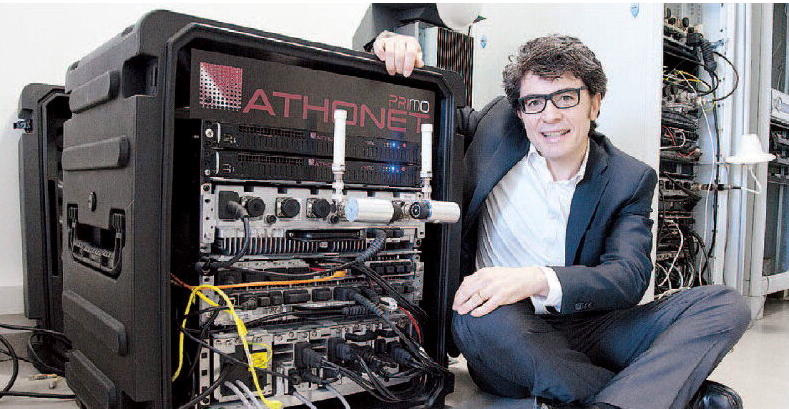
\includegraphics[width=.8\textwidth]{resources/gianluca_primo}\\
		\caption{The CTO, \textit{Gianluca Verin}, with Athonet's main product \textbf{\Quote{PriMo}}\cite{gianluca_primo}}
	\end{figure}
	In 2012, after a disastrous earthquake destroyed all the communication lines in Emilia Romagna, Athonet has reestablished connectivity, thus showing the how PriMo can be used on the field in emergency situations.\\
	Athonet installed PriMo at the top of a school, allowing them to cover the affected area not only for the operators of Servizio Civile but for the citizens as well.\\
	In December 2013, Athonet has been rewarded by Giorgio Napolitano, the then President of the Italian Republic, with a medal for merits for the sustainability in the digital sector.\\
	Lately they have migrated some of their functions to the cloud: by using AWS they have achieved a hybrid product, BubbleCloud, a plug and play solution that allows to locally deploy the physical Edge Nodes while managing them from the AWS cloud.\\
	This small business has much to offer, considering that some of it's competitors are giants like Nokia and Ericsson.\\
	As a proof of the continuous will to improve and for the solution it provides, Athonet has been awarded with four Global Mobile Awards at the GSMA Mobile World Congress, held in February 2019 in Barcelona.
	%todo inserire citazioni
%	https://www.millionaire.it/athonet-la-startup-italiana-che-trionfa-al-mobile-world-congress/#!
%	http://www.ilgiornale.it/news/interni/genio-torna-svezia-soffrire-nella-sua-italia-912407.html

\section{The project}
	It consists in installing and configuring two main software tools, Jira and Confluence, alongside plugins to add more functions and enhance their potentiality.
	However, the most important part of this project is not installing the software, but adapting it to the needs of the company.\\
	As said earlier Athonet my still be small, but it's a growing company, and because of this it needs to give itself some internal rules and specifications to follow when working on a task, communicating with the client or even share internal information to employees.
	Not only for themselves but for clients they work with as well, since most big companies require that their partners have internal regulations, no matter the number of people in the company.\\
	As I will explain in the following chapters Jira is an Issue Tracking System, a software that allows to follow the tasks (like resolving bugs or implementing features) that are related to a project, while Confluence is a software for sharing knowledge, that means sharing internal documents, keeping a wiki, having documentation available and even for customers.\\
	My task was to demonstrate that these tools are what Athonet needs to be a strong an coherent company, where information is always shared and available, while maintaining a history of changes, by creating an environment that suited their needs and that can evolve alongside the company.\\
	To do this I have learned the basics of Agile and Scrum methodologies, how a company operates internally and with their clients and how introducing a new tool may improve the way of working, even if it creates chaos at the beginning.

\section{Document organization}
	This thesis is organized as follows:
	\begin{itemize}
		\item Chapter 1 or \Quote{Introduction}: describes the overall content of this document
		\item Chapter 2 or \Quote{The internship project}: describes in detail the objectives and planning of the internship project
		\item Chapter 3 or \Quote{Agile processes and methodologies}: an introduction to the Agile software development
		\item Chapter 4 or \Quote{Jira and Confluence: the essentials}: describes the most valuable functionalities of Jira and Confluence
		\item Chapter 5 or \Quote{Project implementation}: details how the project has been implemented by dividing it into time periods
		\item Chapter 6 or \Quote{Conclusions}: contains the retrospective of the project, future developments and personal considerations
	\end{itemize}
	

	%!TEX root = ../dissertation.tex
\begin{savequote}[75mm]
This is some random quote to start off the chapter.
\qauthor{Firstname lastname}
\end{savequote}

\chapter{Processi e metodologie dell'agile}


Possibile introduzione del tipo "Before getting into what I have concretely achieved / implemented, let's take a better look at what agile is and how it came to be" (overview)

\section{breve storia dell'agile}
cosa c'era prima dell'agile\\
quando dove e perchè c'era la necessità

\section{il manifesto agile}
i 4 punti fondamentali del manifesto agile

\section{i dialetti / cugini dell'agile}
kanban, etc.

\section{applicazioni dell'agile }
modello spotify (+ altre grandi aziende)\\
e le piccole aziende come athonet come fanno? (misto)

\section{utilità agile}
l'agile può andare a completamente sostituire il resto\\
cosa ne pensano gli utenti

\section{che tipo di agile viene utilizzato da athonet}
misto a causa dei pochi dipendenti che hanno ancora una responsabilità ampia all'interno dell'azienda ma pensano che si possa incorporare agile\\
processi di business


	%!TEX root = ../thesis.tex
\begin{savequote}[75mm]
\hl{If a team couldn’t be fed with two pizzas, it was too big.}
\qauthor{Jeff Bezos}
\end{savequote}

% https://areomagazine.com/2019/04/10/agile-and-the-software-industrys-ideology-problem/ 
%https://www.softwaretestinghelp.com/agile-manifesto/
%https://www.smartsheet.com/comprehensive-guide-values-principles-agile-manifesto

\chapter{Agile Software Development}
\label{chapter_3}

Before getting into the implementation and adaptation of Jira and Confluence, \hl{let's back up a little} and understand the concept of Agile, a Software Development Life Cycle (or SDLC) model.\\
%todo rivedere per bene
SDLCs did not emerge until the 1960s; they are considered to be the oldest formalization of framework.
%The Space Shuttle program, which operationally launched in 1982, used information and processing technologies from the 1960s.
A SDLC refers to the ensemble of activities that compose a software project.\\
It starts with the concepts of understanding the problem as well as the requirements and it ends with the retirement of the system (when there is no more maintenance) or with the cancellation of the project.\\
Small projects (generally for a single person) have a simpler life \hl{cycle: find the problem and write a program to solve it: once the problem has been solved}, the program can be deleted and forgotten.\\
%todo or in larger problems / solved
In larger projects, that require a team to be developed, there must be some explicit rules to set a higher quality for the software.\\
As activities are assigned to different people, it becomes critical that all participants share a common view of the execution of the project.
A SDLC model is a framework providing the ordering and dependencies of life cycle activities, managing these can be a major impact for a successful project and its duration.\\
For example, a change in requirements during implementation may invalidate a substantial amount of work and delay the delivery of the system by several months.
Different life cycle models prescribe different actions to handle such changes\cite{software_lyfe_cycle}.\\
%https://en.wikipedia.org/wiki/Software_development_process
%todo mettere tra virgolette
There are many SDLCs like Waterfall, Prototyping, Iterative and Incremental Development, Spiral Development, Rapid Application Development, and Extreme Programming. (XP). 
%todo modificare immagine
%Font piccolo nell'immagine e nella didascalia. In principio, il font dovrebbe essere a grandezza costante sia nel testo che nelle immagini
\begin{figure}[H]
	\centering
	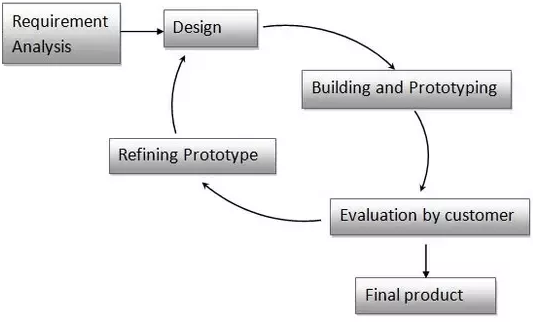
\includegraphics[width=.7\textwidth]{resources/prototype}\\
	\caption{The Prototype model}
\end{figure}
\begin{figure}[H]
	\centering
	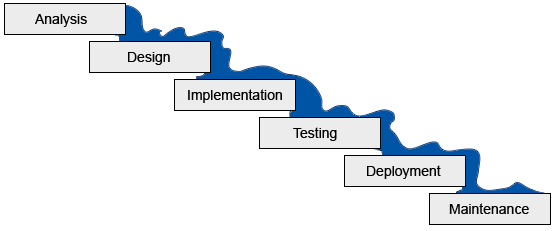
\includegraphics[width=.7\textwidth]{resources/warterfall}\\
	\caption{The Waterfall model}
\end{figure}
%https://www.iso.org/obp/ui/#iso:std:iso-iec:tr:24774:ed-2:v1:en
%todo citare https://www.iso.org/standard/53815.html !!
As the word \Quote{model} suggests, each company may have its own SDLC designed ad hoc for their internal use.\\
This led to the creation of a standard that presents the guidelines for the elements that are most frequently used in describing a process: the title, purpose, outcomes, activities, task and information item.
%todo citare
The ISO/IEC TR 24774:2010: Systems and software engineering -- Life cycle management -- Guidelines for process description\cite{iso_53815}.\\
The complexity and slowness in producing a concrete product in older SDLCs brought the need for a faster and more communicative model.\\
%https://www.tutorialspoint.com/sdlc/sdlc_agile_model.htm
%todo mettere a glossario
%Agile SDLC model is a combination of iterative and incremental process models with focus on process adaptability and customer satisfaction by rapidly and continuously deliver of working software product.
%todo trovare immagine a risoluzione migliore
\begin{figure}[H]
	\centering
	
\includegraphics[width=\textwidth]{resources/BffFTn_CAAAEvGn}\\
	\caption{\textit{Redmine}'s logo}
\end{figure}
This chapter describes the most fundamental points of the Agile method, how it started and the adaptations that derived from it, like Scrum.
At the end, it also explains how Athonet's adaptation of the Agile life cycle works.

\section{The need for a new Software Life Cycle}
	The decade of 1990 represented a very important turning point for the digital industry.
	Computers were spreading everywhere and the software companies faced the so-called application development crisis.\\
	The problem was that businesses moved too fast and within the space of three years, requirements, systems, and even entire businesses were likely to change. 
	It meant that a lot of software ended up being incomplete or canceled halfway and the ones that made it through, even if they fulfilled the original objectives of the client, may not meet all the business needs\cite{agility-beyond-history}.
%	https://hackr.io/blog/sdlc-methodologies
	SDLC models can be of two types:
	\begin{itemize}
		\item Iterative: enhances the evolving versions until the complete system is implemented and ready to be deployed
		\item Incremental: the product is designed, implemented and tested incrementally until it is finished
	\end{itemize}
	One of the most characteristic models used before Agile was the Sequential model (or Waterfall).
	The waterfall model became very famous because it has many strong points as:
	\begin{itemize}
		\item Uses clear structure
		\item Determines the end goal early
		\item Transfers information well
	\end{itemize}
	On the other hand, it became obsolete when projects started to be more dynamic and complex.
	Some of it's disadvantages are:
	\begin{itemize}
		\item Makes changes difficult
		\item Excludes the client and/or end user
		\item Delays testing until after completion
	\end{itemize}
	The excessive documentation, the forceful binding to the unchangeable decisions made early in the project and the little communication with the client brought to the need of a new model that prioritizes the product and the stakeholders over bureaucracy.\\
	Those things frustrated people like Jon Kern, an aerospace engineer in the 1990s that with other figures from different industries \Quote{were looking for something that was more timely and responsive}, as he noted.
	He was one of 17 software leaders that started meeting informally and talking about ways to develop software in a simpler way without the excess of documentation and other strict rules.\\
	These talks led to the now famous Snowbird meeting (in Utah, February 2001), when the Agile Manifesto was written down and published.

%
\section{The Agile manifesto}
	The Agile Manifesto is a brief document built on four foundational values and twelve supporting principles for Agile software development\cite{agilemanifesto}.\\
	The four values written on the official website\cite{agile_official} are:
	\begin{itemize}
		\item \textbf{Individuals and interactions} over processes and tools
		\item \textbf{Working software} over comprehensive documentation
		\item \textbf{Customer collaboration} over contract negotiation
		\item \textbf{Responding to change} over following a plan
	\end{itemize}
	The responsiveness of people and embracing the importance of changes are the fundamentals of Agile.
	Although documentation is secondary, it's important to note that Agile streamlines documentation and does not eliminate it.\\
	These twelve principles emphasize things like \Quote{early and continuous delivery of valuable software” and “continuous attention to technical excellence}, and are: 
	\begin{enumerate}
		\item Our highest priority is to satisfy the customer through early and continuous delivery of valuable software.
		\item Welcome changing requirements, even late in development. Agile processes harness change for the customer's competitive advantage.
		\item Deliver working software frequently, from a couple of weeks to a couple of months, with a preference to the shorter timescale.
		\item Business people and developers must work together daily throughout the project.	
		\item Build projects around motivated individuals. Give them the environment and support they need, and trust them to get the job done.
		\item The most efficient and effective method of conveying information to and within a development team is face-to-face conversation.
		\item Working software is the primary measure of progress.
		\item Agile processes promote sustainable development. The sponsors, developers, and users should be able to maintain a constant pace indefinitely.	
		\item Continuous attention to technical excellence and good design enhances agility.
		\item Simplicity--the art of maximizing the amount of work not done--is essential.
		\item The best architectures, requirements, and designs emerge from self-organizing teams.
		\item At regular intervals, the team reflects on how to become more effective, then tunes and adjusts its behavior accordingly.
	\end{enumerate}
	All of them are important but, in my opinion, the ones that add the most value to the Agile line of thought and that differentiate it from the other methods are 2, 4 and 6: they represent the intent of placing the product and the customer above everything else, allowing the use of small informal meetings (even if the decisions should be recorded) and the easy change of requirements because the client is always involved, even as an end user (tester).\\
	Each Agile methodology applies the four values in different ways.
	However, all of them rely on these values to guide the development and delivery of high-quality, working software\cite{4-values-of-the-agile-manifesto}.

\section{Agile's little big cousins}
	While Agile's manifesto contains values and principles, these are not prescriptive.
	In fact the manifesto does not outline specific processes, procedures or best practices.
	The goal is not to develop a rigid framework but rather create a mindset for software development.
	Agile is a blanket term that describes a set of software development principles.\\
	There are many methodologies that derive from Agile's thinking, the most famous ones, according to the annual survey\cite{state-of-agile} from VersionOne's team are:
	\begin{itemize}
		\item Scrum
		\item Scrumban
		\item Kanban
		\item Extreme Programming (XP)
	\end{itemize}
	The essence of Scrum is being agile (fast): a small team that is highly flexible and adaptive.
	\begin{figure}[H]
		\centering
		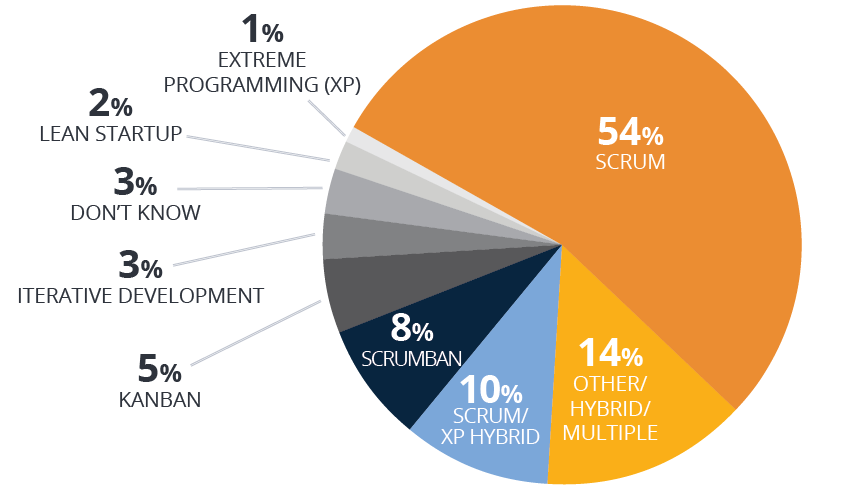
\includegraphics[width=.8\textwidth]{resources/agile-usage-chart}\\
		\caption{The Waterfall and Prototype SDLC models}
	\end{figure}

	%todo modificare immagine
	\begin{figure}[H]
		\centering
		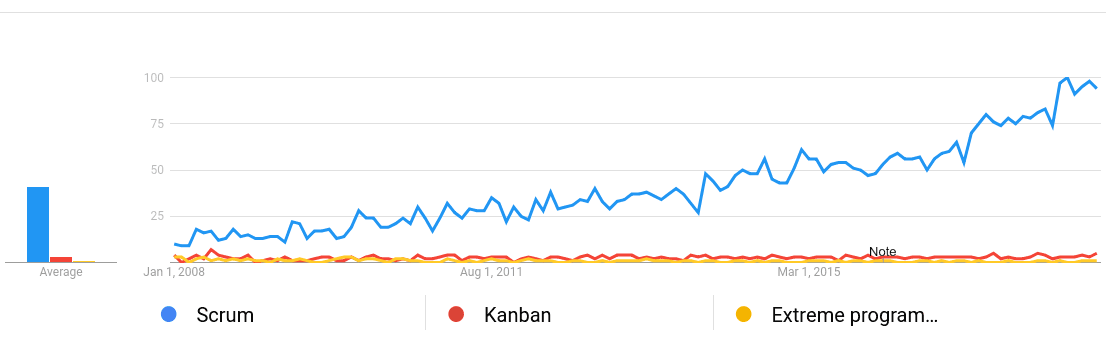
\includegraphics[width=\textwidth]{resources/trends}\\
		\caption{The Waterfall and Prototype SDLC models}
	\end{figure}
	This survey is quite interesting because it provides information from small and big real companies that want to share their experience.
	A very important fact to be noted is that although Technology companies are the ones that mostly participated to the survey, there are other industries that use Agile and are interested in sharing their experience.
	\begin{figure}[H]
		\centering
		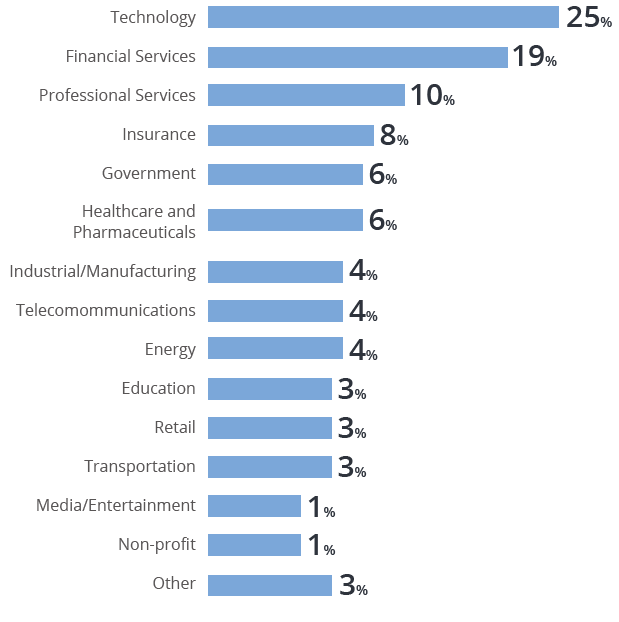
\includegraphics[width=.8\textwidth]{resources/Untitled_2}\\
		\caption{The Waterfall and Prototype SDLC models}
	\end{figure}
	It states that for the year 2018 (which marked their 13th annual report) the reasons for adopting Agile were productivity, improving team morale, reducing product risk (with a lesser percentage than the previous year) and about reducing project costs.\\
	The measures of success mostly cited by the respondents were customer, or user, satisfaction and business value.\\

	%todo Qui devi elencare, e mettere un link alla figura con le percentuali. Il testo dovrebbe contenere tutte le informazioni necessarie per capire il tuo discorso, e le figure servono come chiarimento. Ciascuna figura dovrebbe essere indipendente, nel senso che tra immagine e didascalia si dovrebbe riuscire a capire tutto. 

	According to these companies, the benefits of adopting Agile are:
	\begin{figure}[H]
		\centering
		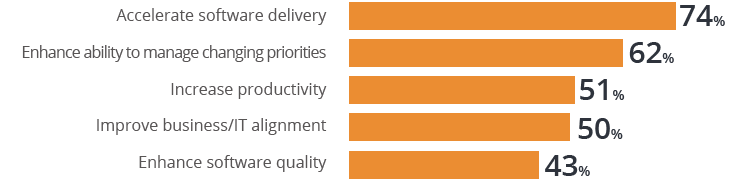
\includegraphics[width=.8\textwidth]{resources/Untitled}\\
		\caption{The Waterfall and Prototype SDLC models}
	\end{figure}

	Also the questionnaire contained a question about what are the recommended Agile project management tools.
	
	%todo modificare immagine
	\begin{figure}[H]
		\centering
		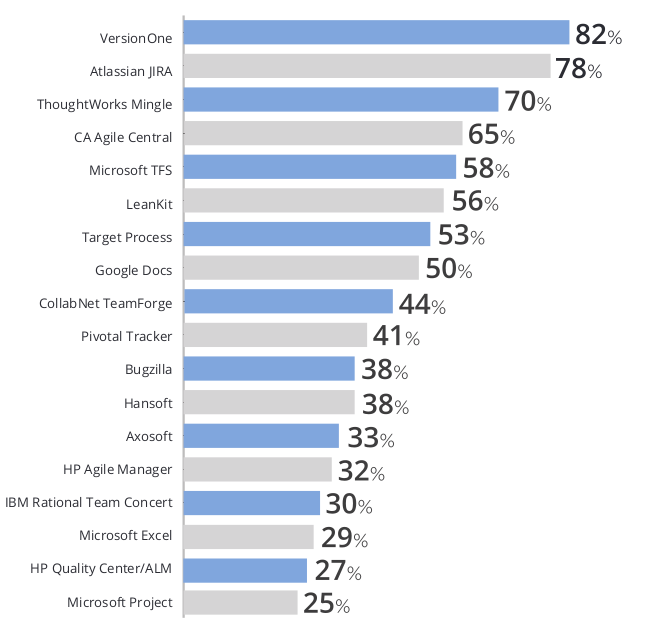
\includegraphics[width=.8\textwidth]{resources/Screenshot}\\
		\caption{The Waterfall and Prototype SDLC models}
	\end{figure}

	As we can see Jira is the second most recommended one.

	\begin{figure}[H]
		\centering
		
\includegraphics[width=.8\textwidth]{resources/Untitled_4}\\
		\caption{The Waterfall and Prototype SDLC models}
	\end{figure}

\section{Agile in practice}
\hl{Briefly describe how some companies use Agile: Spotify / Netflix / Amazon}

% SPOTIFY
%https://medium.com/@media_75624/exploring-key-elements-of-spotifys-agile-scaling-model-471d2a23d7ea
%https://medium.com/productmanagement101/spotify-squad-framework-part-i-8f74bcfcd761

% AMAZON
%https://www.forbes.com/sites/stevedenning/2019/06/02/how-amazon-became-agile/

% MICROSOFT
%https://www.forbes.com/sites/stevedenning/2015/10/27/surprise-microsoft-is-agile/

% NETFLIX
%https://smartbear.com/blog/develop/5-lessons-agile-teams-can-learn-from-netflix/
%http://www.agileadvice.com/2018/03/02/profiles/a-case-study-of-netflixs-high-performance-culture/

%LSD (Lean Software Development)
%This methodology is an adaptation of the Toyota lean manufacturing principles to software development. It was introduced in 2009 by Marry and Tom Poppendieck in their book "Lean Software Development: An Agile Toolkit."

\section{The roles in Agile}
	A distinctive characteristic of the Agile methodology is it's definition of roles: they are not positions, any given person takes on one or more roles and can switch them over time, and any given role may have zero or more people in it at any given point in a project\cite{agileRoles}.
	The ideal team is considered to be composed of five or six people.\\
	These roles are:
	\begin{itemize}
		\item Team leader: team coach or project lead in other methods (Scrum-master e.g.), he is responsible for facilitating the team, obtaining resources for it, and protecting it from problems
		\item Product owner: an executive or key stakeholder, the Product Owner has a vision for the end product and a sense of how it will fit into the company’s long-term goal
		\item Team member: developer or programmer, is responsible for the creation and delivery of a system
		\item Stakeholder: any other person that has direct or indirect interest in the project
	\end{itemize}

%https://www.dummies.com/careers/project-management/agile-project-management-artifacts/
%https://www.atlassian.com/agile/project-management/metrics
%https://www.cognizant.com/services-resources/Services/Cognizant-Agile-Metrics-What-You-Need-to-Want-to-and-Can-Measure.pdf
\section{Time cycles and metrics}
	\hl{COMPLETE}\\
	Scrum teams coordinate development into time-boxed sprints.
	Outside the sprint, teams organize and forecast the amount of work that can be concluded.
	The goal is to have all the forecasted work completed by the end of the sprint.\\
	There are metrics used to track the completion of tasks, these are called burndown reports.
	\begin{figure}[H]
		\centering
		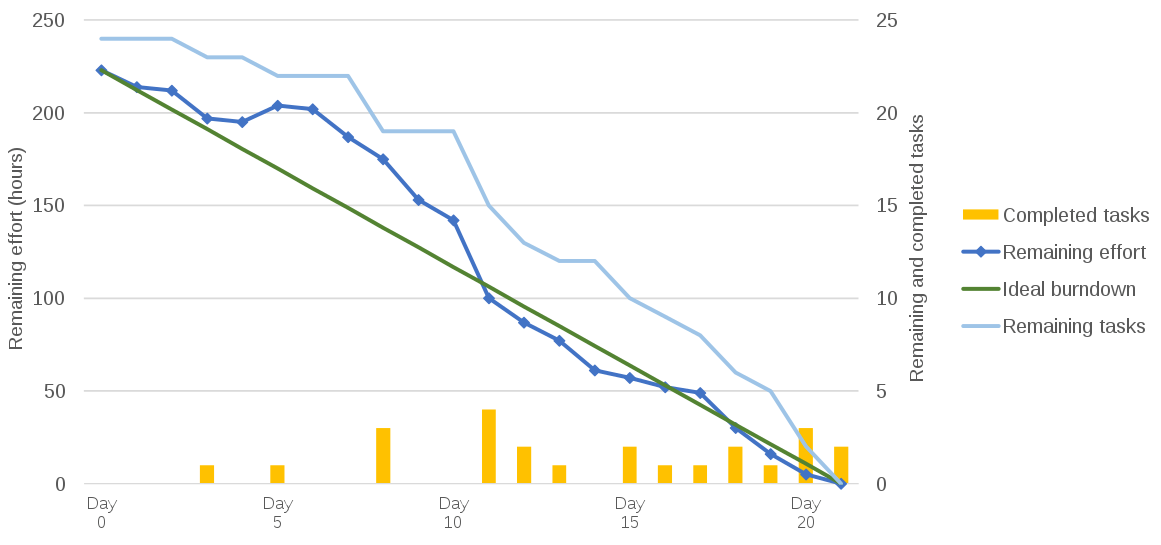
\includegraphics[width=\textwidth]{resources/burndown}\\
		\caption{The Waterfall and Prototype SDLC models}
	\end{figure}
	The x-axis represents time, and the y-axis refers to the amount of work left to complete, measured in either story points or hours.\\
	The sprint is one of the most important time periods in Agile, the other principal ones, according to Atlassian's Agile Coach\cite{epics-stories-themes} are:
	\begin{itemize}
		\item Stories: short requirements or requests written from the perspective of an end user
		\item Epics: large bodies of work that can be broken down into a number of smaller tasks (called stories)
		\item Initiatives: collections of epics that drive toward a common goal
		\item Themes: large focus areas that span the organization
	\end{itemize}
	\begin{figure}[H]
		\centering
		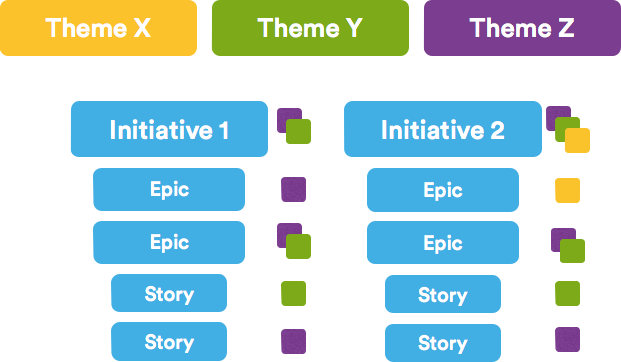
\includegraphics[width=\textwidth]{resources/Themes}\\
		\caption{The Waterfall and Prototype SDLC models}
	\end{figure}
	
%	todo prendere da questo sito https://www.atlassian.com/agile/project-management/epics-stories-themes
	
%https://leankit.com/learn/agile/what-are-the-disadvantages-of-agile/
\section{Disadvantages of Agile Software Development}
	Despite the benefits offered by the Agile model, transition a company's way of working to it is not that easy and if done wrong it may make damage instead of good.
	According to the American entrepreneur Adam Fridman, here are the drawbacks\cite{massive-downside-of-agile} of Agile:
	\begin{enumerate}
		\item Less predictability: developers may not be able to quantify the full extend of the required effort
		\item More time and commitment: a constant interaction, with many face-to-face conversations, is required
		\item Greater demands on developers and clients: extensive user involvement that impacts the quality and success of the project
		\item Lack of necessary documentation: new members that join the team may need more time to understand the project
		\item Project easily falls off track: if a consumer's feedback or communications are not clear, a developer might focus on the wrong areas of development
	\end{enumerate}
	
\section{What Agile variant Athonet uses}
	As many small companies, Athonet will not strictly use one Agile implementation.
	This is also due because of the nature of their product that is not released in simple software patches but it presents itself in a more monolithic version.
	After a research for the available software development life-cycle tools on the market, they chose to try Atlassian's Jira in tandem with Confluence.\\
	As I will say in \Chapref{chapter_5}, the managers liked the idea of Kanban because it allows the employees to come in the morning and choose what they want to work on from the backlog without giving them a two week period of time but letting them complete the tasks in time for the following release.
	But they also liked the idea of having a tool that could transition from a type of project to another in case they want to start applying stricter rules in the future.
	%todo immagine doppia modificare
	\begin{figure}[H]
		\centering
		
\includegraphics[width=\textwidth]{resources/Dilbert_Training_Agile_Programming}\\
		\caption{The Waterfall and Prototype SDLC models}
	\end{figure}


	%!TEX root = ../thesis.tex
\begin{savequote}[75mm]
Nulla facilisi. In vel sem. Morbi id urna in diam dignissim feugiat. Proin molestie tortor eu velit. Aliquam erat volutpat. Nullam ultrices, diam tempus vulputate egestas, eros pede varius leo.
\qauthor{Quoteauthor Lastname}
\end{savequote}

\chapter{Projet implementation}

This chapter is the core of this document and describes the way that this project has been implemented according to the work plan described in Chapter 2.

It is structured in four main sections, each representing a time period:
\begin{enumerate}
	\item Learning stage - RIVEDERE NOME
	\item Implementation
	\item Testing
	\item Feedback
\end{enumerate}

%todo rivedere tutto
\section{Learning stage - CAMBIARE NOME}

	This phase corresponds to the first two weeks of the internship.
	As described in the work plan in this first period the main task was to understand what the tools are.
	At first I have started to search information about Jira and Confluence on Google.
	%todo aggiungere riferimento a official documentation
	The first tools I have started researching was Jira, and the official documentation is very well organized.
	\begin{figure}[H]
		\centering
		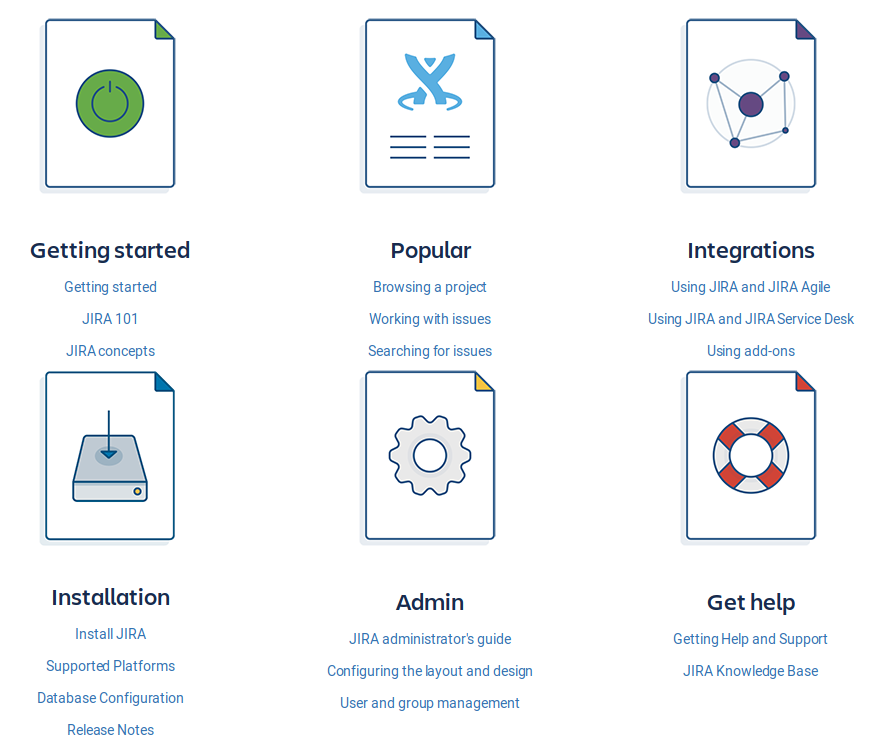
\includegraphics[width=1\textwidth]{resources/jira_documentation}\\
		\caption{Screenshot of the Jira Documentation homepage from the Atlassian Support website}
	\end{figure}
	This documentation is very easy to navigate because it versioned for each release, major and minor, of the software, plus it contains links to related pages.	
	If there is a reference about a Confluence webpage, this is added as a link.
	Vice versa on the Confluence documentation, if there is a Jira reference, it links to the latter's documentation.	
	Both Jira and Confluence have a bug reporting and issue tracking section in their documentation.
	\begin{figure}[H]
		\centering
		\includegraphics[width=1\textwidth]{resources/confluence_documentation_issues}\\
		\caption{The issues related with Jira and Confluence are handled by a dedicated Jira Cloud instance}
	\end{figure}
	If a webpage in the documentation is related to an issue, the latter is showed at the end of the page with its status and a link to its dedicated section. %todo rivedere parola userbase
	The Confluence and Jira documentation are both written and hosted using Confluence, showing how powerful can be this tool for handling a wiki for such a complex software that has a large userbase.
	Confluence's documentation is structured like Jira's, very easy to access and consult.	
	Another bonus is that it is public and free to consult, despite the software is not.
	This may seem like an obvious choice but not all vendors do it: RedHat for example let's you consult their documentation only if you log into the website.
	
\section{Initial installation and configuration}
	
	During the second week, while studying the documentation I went ahead and started configuring the software.
	In order to install the Atlassian tools I was given a CentOS VM with 512GB of storage and 32GB of RAM.
		
	%todo logo centos
	
	To connect with the remote machine, which was in a controlled testing environment, I used Remmina, a remote desktop client for Linux operating systems.
	This allowed me to easily connect to the machine to install software or to troubleshoot it in case of a failure.
	As for the previous phase, the first software I installed was Jira, by following the official documentation.
	%https://confluence.atlassian.com/adminjiraserver/installing-jira-applications-on-linux-938846841.html
	\begin{figure}[H]
		\centering
		
\includegraphics[width=1\textwidth]{resources/jira_installation}\\
		\caption{The issues related with Jira and Confluence are handled by a dedicated Jira Cloud instance}
	\end{figure}
	
	% todo aggiungere riferimento a paragrafo
	As told in ...aggiungere riferimento... Jira requires a database to work properly.
	For the first installation, which was made for testing purposes, the embedded H2 database was enough.
	
	%todo aggiungere immagine prima pagina di jira appena installato
	
	The first thing that I have done after the installation was getting acquainted with the interface and understanding how Jira's components interconnect with each other.
	To do this I have created some mock projects that I filled with issues, it is here that I understood the concept of Board in Jira.
	Experimenting with workflows was one of the most important things to do, because these are fundamental in an issue tracking system's configuration and are strictly connected to the concept of Board.
	
	% todo inserire immagine di board
	
	After understanding the fundamentals of this software and getting to know it's basic features, I went ahead and installed Portfolio.
	
	%todo aggiungere riferimento
	This plugin, as told in ...aggiungere riferimento... helps visualizing the issues on a roadmap, which was one of the most important requirements.
	
	Installing Portfolio was easy, I just followed the instructions on the documentation to install the latest version of the plugin.
	
	%todo inserire immagine di portfolio
	
	After installing Portfolio and creating plans for my mock up projects, I have chosen to install Service Desk, to complete the configuration of the Jira instance.
	As earlier I have followed the documentation on Jira's website.
	As described in ...aggiungere riferimento... this piece of software is used to communicate with the clients and having a portal from which a client can find information and request assistance with a product.
	The first thing I tested after installing this software was creating a portal and see from the point of view of a client how this can be able to open an issue and what type of issues he may have access to.
	
	%todo inserire immagine Service Desk
	
	Not long after I have installed Confluence, and like Jira, I have used it's embedded database.
	Both software run on the same system, and their services are offered on port 8080 and 8090 respectively for Jira and Confluence.
	Soon after I connected the software together and I tested it out by creating a knowledge base for a Service Desk project and a documentation space for a Software project.
	Confluence was easier to get familiar with, so after creating some mock spaces related to the projects that were in Jira at the time, I moved on.

	At this point there was a change in the requirements that were given to me by the tutor.
	Contrary to what he said, the IT department opted to use GitLab instead of BitBucket because the developer know it better and for their usage tier there is no billing.
	So it's free.
	
	This meant that there would be a tool less that needed to be installed, but I had to understand how to link Jira's functionalities to those offered by GitLab.
	
	Connecting these tools together means that a developer can interact with Jira's issues in a project by typing it's ID in the messages that he uses for commits, comments, merge requests and so on.
	
	Fortunately GitLab's documentation had a dedicated page that allowed me to configure both tools.
	
	% https://docs.gitlab.com/ee/user/project/integrations/jira.html
	
	This functionality though allows GitLab to interact with Jira's default workflows.	
	If the licence for GitLab's hosted version is not Premium (or Silver for the online one) there is no interaction from Jira to GitLab.
	
	% https://docs.gitlab.com/ee/integration/jira_development_panel.html
	
	There is no 1:1 project mapping from GitLab to Jira, a commit message in the repository may reference multiple Jira issues from different projects.
	
	Later ...aggiungere riferimento... I will talk about installing a plugin that allows these tools to be better connected.
	
	After understanding the potentiality of this connection I went on and set up a small demo that touched all the things that I have covered in the first two weeks of the internship.
	Since my tutor wasn't available for a few days so I took the liberty to customize the environment by changing the colors and logos in the interface, putting Athonet's.
	
	% todo inserire immagine di interfaccia customizzata
	
	During the meeting I have taken with the tutor, he said that he liked the work I have done and that it was time for more elaborate mock projects in order to present the tools' functionalities to other company figures.
	
	After that I have deleted the mock projects from Jira and the related spaces in Confluence to ask the IT department for a snapshot of the VM I was working on.
	
	This allowed me to have a milestone / baseline.
	A deliverable that I was able to use as a secure point in time in which I could go back if anything after went wrong.
	
\section{First realistic mock projects and feedback}
	
	The fourth week of the internship I was ready to implement more realistic projects in Jira, connecting them to Confluence providing them with documentation and creating a link with GitLab.
	The objective was to have a working demo that could be shown to various members of Athonet for them to understand how these software can be used in their departments.

	In Jira I have created the projects EPC and Dashboard, both Software projects, while in Confluence I have created the spaces EPC Documentation and Dashboard Documentation.
	Also in Jira I have created an Athonet Internal Wiki project, to show how Service Desk could be useful for sharing internal documents between employees.
	
	For the first project I have implemented a more articulate workflow that resembles the realistic evolution of an issue inside the company and customized the menus that allow the creation of an issue.
	Later these will be revised because in this stage I did not have the information about what an issue requires to have in Athonet's case. 
	
	As I continued working on the mock projects and creating issues, I noted down all the most important customization that an administrative user can use to set up the software, not only for Athonet's specific purposes but in general.
	
	To make the project more realistic I have created three user groups, besides the default ones, to which I have assigned three users each:
	\begin{itemize}
		\item Management
		\item Verification
		\item Developers
	\end{itemize}
	
	Every group had various permissions; that allowed me to demonstrate how basic security works in these tools.
	
	
	
	--------------------------------------
	
	understanding what an issue is, what a project is, how a project is different than a product, understanding what a workflow is and how it applies to different projects
	
	Installation of Service desk.
	
	Installation of Confluence, using H2 database.
	
	
	Interconnecting Jira and Confluence.
	Creating a first knowledge base.
	
	
	first requirement change, using gitlab
	connecting gitlab
	utilizzare gitlab (con account personale su server aziendale e progettini di mock) per effettuare transizioni automatiche delle issue (spiegare correlazione tra progetti in gitlab e in jira)
	
	customizing the user interface while waiting for a meeting with the tutor
	
	
	snapshotting the machine
	parlare di milestone / baseline\\
	
	
	
	
	% todo tenere per dopo, prima parlare di intallazione di Jira con db preinstallato
	Before installing anything thought it was necessary to correctly set up a database.
	This was discussed with the tutor and the IT department, which opted for the latest stable distribution of PostgreSQL.

	Installing postgres wasn't written on the work plan but it was included in ... 
	
	%todo inserire logo postgresql
	
	The reason for it is because it's free and open source, besides, other members of the IT department have used it and are familiar with it.
	
	After installing PostgreSQL I was able to make a clean installation of Jira.
	
	








	\subsection{First configuration}
		interconnessione tra i tool
	
	\subsection{Understanding the products}
		creazione di progetti di mock\\
		interconnetterli\\
		capire il workflow delle issue\\
		utilizzare gitlab (con account personale su server aziendale e progettini di mock) per effettuare transizioni automatiche delle issue (spiegare correlazione tra progetti in gitlab e in jira)

	\subsection{Requirements change}
		non usare bitbucket ma gitlab\\
		visto il grosso ammontare di elementi customizzabili è stato necessario scremare le cose e capire cosa si poteva facilmente aggiungere e cosa lasciare per dopo\\
		abbellimento dell'environment
		
		%todo logo dei due prodotti

	\subsection{Customizing the user interface}
		a causa della poca disponibilità in questo primo periodo di marco e paolo che utilizzeranno questo tool in maniera intensiva rispetto al tutor, ho fatto un task secondario come quello della personalizzazione dell'interfaccia grafica
	
		%todo immagini interfaccia grafica prima e dopo
	
	\subsection{snapshot della macchina per salvare il lavoro svolto per ora}
		parlare di milestone / baseline\\
		come le ho pensate nel piano di lavoro

\section{First realistic mock projects and feedback}

	This phase corresponds to ... in the work plan

	\subsection{The projects}
		idee del tutor\\
		prime demo con lui per capire se questo tool effettivamente copre le necessità di base dell'azienda
		
	\subsection{Integrating with GitLab}
		in questo periodo vista la scarista di opzioni di gitla nativo si è scelto di usare un plugin\\
		(decontestualizzare il tempo, a posteriori, ragionando per milestone)\\
		visto integrazione nativa\\
		scelta di utilizzare un plugin\\
		costa ma è migliore (descrivere da quale punto di vista)
	
	\subsection{First meetings to present the progress}
		primo feedback e discussioni di come può evolvere il progetto e come può essere applicato ai loro workflow\\
		riflessioni personali: a questo punto sto rispettando il piano di lavoro iniziale? sono in ritardo / anticipo?
	
	\subsection{New requirements change}
		giustificare --> dopo fase di studio / riscontro\\
		cosa può essere implementato subito, cosa no, come viene usato\\
		campi e workflow custom\\
		mapping tra processi jira e interni (sprint)
	
	\subsection{Documentation}
		scrittura della bozza di documentazione e passaggio della documentazione in confluence
		
	\subsection{New snapshot of the machine}
		nuova baseline / milestone

\section{Transitioning to production}

	This phase corresponds to ... in the work plan

	After the approval for using the tools by other departments (R\&D) it's time to transition it / move it to production
	
	\subsection{Migrating data from Redmine}
		tool automatico di migrazione
		collegamento con redmine, lo fa in maniera automatica
		e se va male? c'è sempre lo snapshot
	
	\subsection{First non mock projects}
	
	\subsection{Fine tuning of the final product}
		interazione con le persone
		in base alle necessità degli utenti e di come lo usano faccio minime modifiche in produzione
		miglioramento della documentazione
	
	\subsection{How are these tools being used}
		è veramente agile? 
		è un dialetto?
		è un misto?
		perchè athonet lo sta usando in questo modo?

\section{Final feedback and what else could be implemented in the future}

	This phase corresponds to ... in the work plan

	\subsection{Final feedback from the users}
		feedback da parte del tutor
		
		feedback da responsabile strategia aziendale (gl)
		feedback da responsabile del prodotto (aka product ownner / hesham)
		feedback da responsabile sviluppo + testing
			
		feedback da parte di tutti gli utenti
	
	\subsection{What Athonet plans to do with these new tools}
		arrivare ad utilizzare agile in maniera rigida?
		continuare a fare misto?

	%!TEX root = ../thesis.tex
\begin{savequote}[90mm]
	Scrum means ``Waterfall but we don't have time for analisys''\\
	Kanban means ``Scrum, but we don't have time for Sprint planning''\\
	Agile means ``We have no process but we do use Jira extensively''
	\qauthor{\href{https://twitter.com/mikeveerman}{@mikeveerman} on Twitter}
\end{savequote}

\chapter{Projet implementation}
\label{chapter_5}
	This chapter is the core of this document and describes the way that this project has been implemented according to the planning described in \Chapref{chapter_2}.\\
	It is structured in four main sections that go over the main time periods presented in the \Quote{Piano di Lavoro} document.\\
	Since the scope of the project was to create a demo environment to show the capabilities of Jira, Athonet has bought ten user licenses for Jira Software, ten for Service Desk and ten for Confluence.\\
	As described in Atlassian's documentation\cite{compare-atlassian-cloud-vs-server}, these tools have three installation options:
	\begin{itemize}
		\item \textbf{Cloud}: hosted on their infrastructure
		\item \textbf{Server}: download and install on a local network
		\item \textbf{Data Center}: download and install for a large infrastructure
	\end{itemize}
	Because of Athonet's policies about storing internal data in the cloud, the IT department opted for an on premise, Server, installation.
	This kind of installment requires a one time payment for the software while the subsequent fees will be for support.
\section{Learning phase}
	This phase corresponds to the first two weeks of the internship.
	As described in the \Quote{Piano di Lavoro}, the main task in this first period  was to understand what the tools are and what they can do.
	The first important thing to do was to acquire knowledge on Jira and Confluence by researching them on the Internet.
	The first one I have started researching was Jira, this brought me to the official documentation\cite{jira_docu}, which is very well organized.
	\begin{figure}[H]
		\centering
		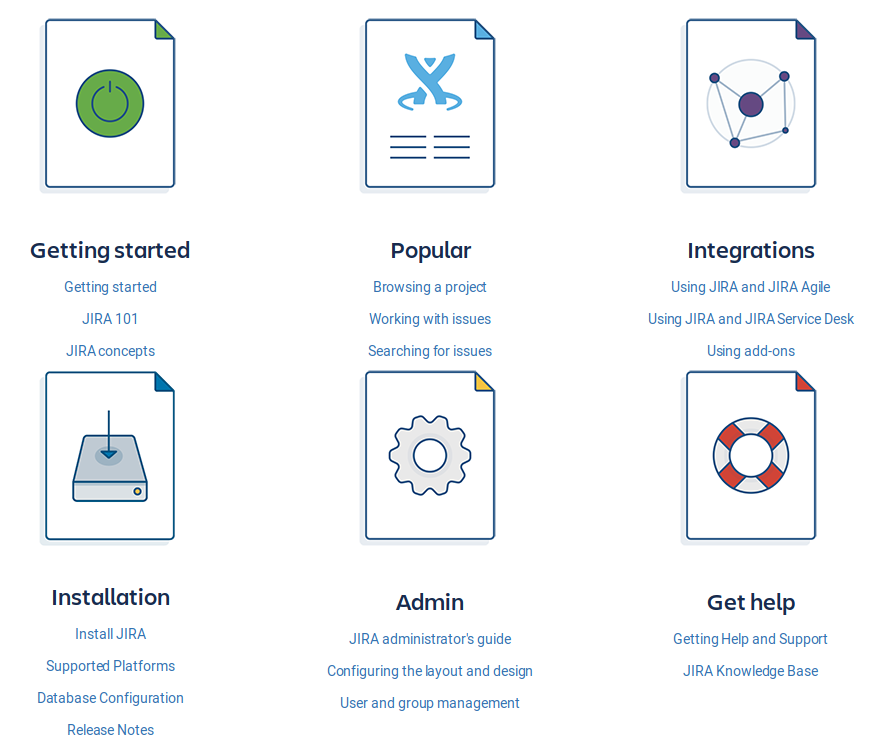
\includegraphics[width=1\textwidth]{resources/jira_documentation}\\
		\caption[Screenshot from Jira's Documentation page]{Screenshot of the sections from Jira's Documentation homepage from the Atlassian Support website}
	\end{figure}
	It is very easy to navigate because it's versioned for each release, major and minor, of the software, plus it contains links to related pages, including Confluence's documentation and Atlassian's blog.
	As said in \ref{sec:atlassian_community} both Jira and Confluence have a bug reporting and issue tracking section in their documentation.
	If a web page is related to an issue, this is showed at the end of the page with its status and a link to its dedicated section.\\
	The Confluence and Jira documentation are both written and hosted using a Confluence instance, showing how powerful can be this tool for handling a wiki for such a complex software that has a large userbase.\\
	Confluence's documentation is structured like Jira's, easy to access and consult, other than being public and free to read, despite the software are not.\\
	The second half of the first week was dedicated to configuring the environment.
	The IT department has chosen to create an instance of the Atlassian's software on a \gls{CentOS}\glsadd{CentOS} \gls{Virtual Machine}\glsadd{Virtual Machine} (VM) with 512GB of storage and 32GB of RAM, connected to a special testing network domain for internship students.
	The \gls{Remmina}\glsadd{Remmina} was used to remotely connect to the given VM.
	\begin{figure}[H]
		\centering
		
\includegraphics[width=.5\textwidth]{resources/centos_logo}\\
		\caption{Logo of the CentOS Linux distribution}
	\end{figure}
	
\section{Initial installation and configuration}	

	Since the exhaustiveness of the documentation, the installation phase was anticipated so that there could be a more hands on approach.
	As for the previous phase, the installation of Jira was done by following the dedicated article on the official documentation\cite{installing-jira-applications-on-linux}.	
	\begin{figure}[H]
		\centering
		
\includegraphics[width=.9\textwidth]{resources/jira_installation}\\
		\caption{Screenshot from the installation page of Jira in Atlassian's documentation}
	\end{figure}
	To store all the information regarding projects, users, etc., Jira needs a database.
	For the first installation, intended to be used in a testing manner, the embedded \gls{H2 database}\glsadd{H2 database} was enough.
	It's important to note that the documentation says the H2 database is not suitable for production environments\cite{accessing-jira-s-h2-embedded-database}.
	The first thing done after the installation was getting acquainted with the interface and understanding ho Jira's components interconnect with each other.\\
	In order to do this it was necessary creating some mock projects and filling them with issues.
	Here is where the concept of Board come out in Jira.\\
	Boards and workflows are very tied notions.
	Experimenting with workflows was one of the most important things to do, because these are fundamental in an Issue Tracking System's configuration and are strictly connected to Boards.
	\begin{figure}[H]
		\centering
		\makebox[\textwidth][c]{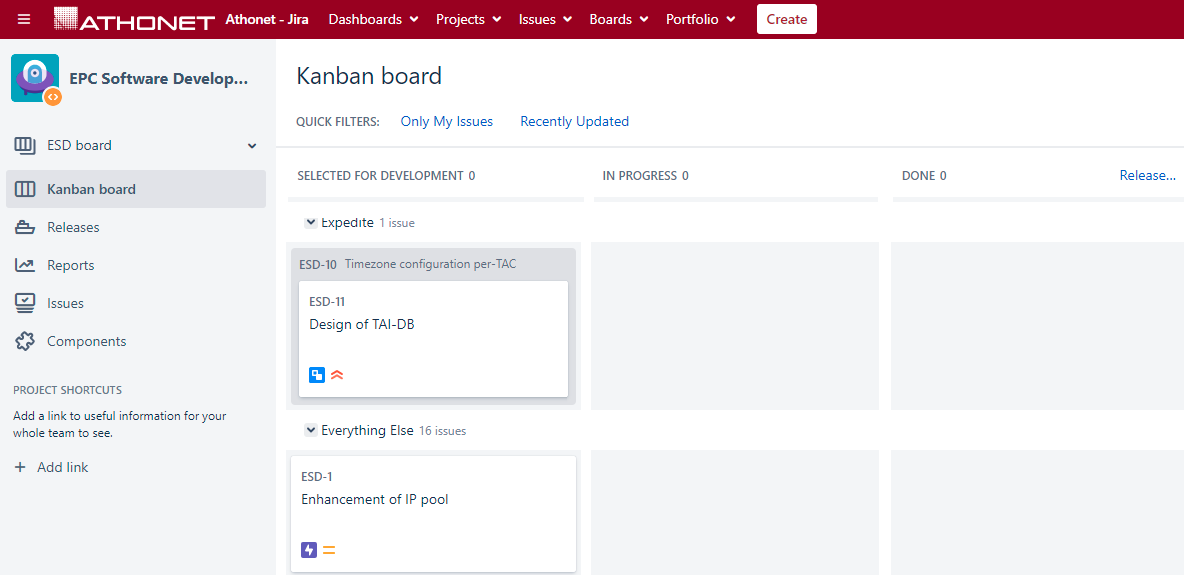
\includegraphics[width=1.2\textwidth]{resources/UntitledA}}%
		\caption{Kanban board from a Jira project}
	\end{figure}
	Installing Portfolio was the step that came after understanding the fundamentals of Jira and getting to know its basic features.
	This plugin, as told in \ref{subsec:portfolio} helps visualizing the issues on a roadmap, which was one of the most important requirements: \textit{O05}.\\
	As per the previous installation, Portfolio's was done by downloading and embedding the binary into Jira's instance.
	\begin{figure}[H]
		\centering
		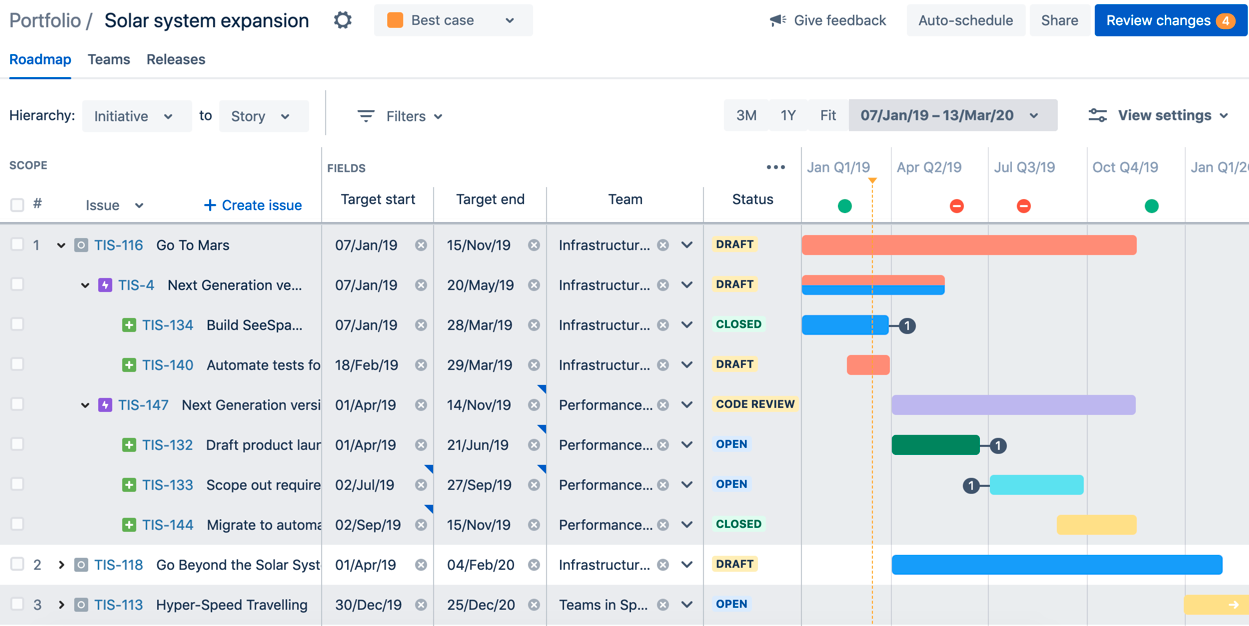
\includegraphics[width=\textwidth]{resources/portfolio}\\
		\caption[Screenshot of roadmap in a Jira Portfolio project]{Screenshot of roadmap in a Jira Portfolio project\cite{portfolio}}
	\end{figure}
	\begin{figure}[H]
		\centering
		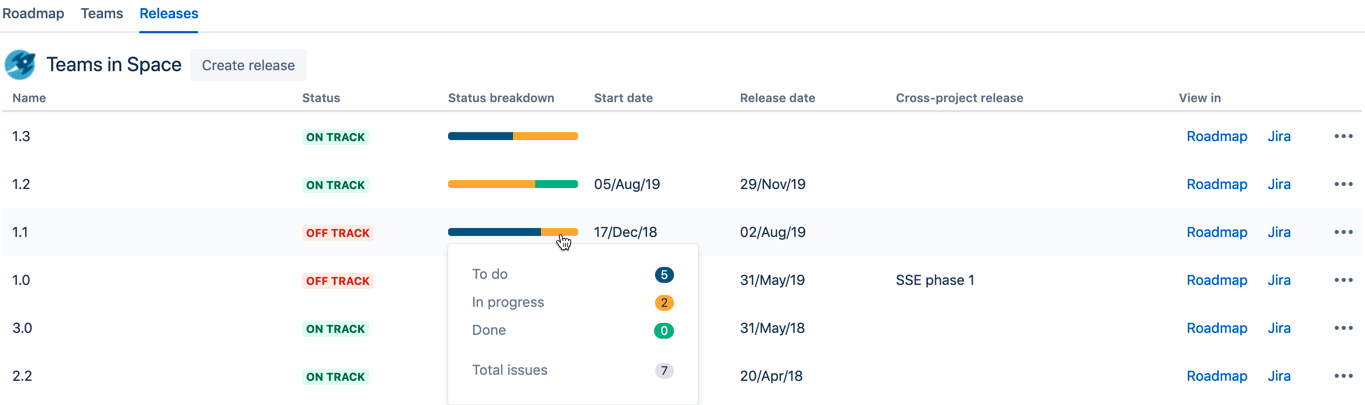
\includegraphics[width=\textwidth]{resources/IPS}\\
		\caption[Screenshot of releases in Jira Portfolio project]{Screenshot of releases in Jira Portfolio project\cite{portfolio}}
	\end{figure}
	The CTO of the company and PriMo's product owner were interested in the possibility of using a real time roadmap to keep track of the work done while not going as in deep as seeing the tasks assigned to each developer.\\
	After installing this plugin and creating plans for the previously created mock up projects, the next software installed was Jira Service Desk, to complete the configuration of the Jira instance.
	As described in \ref{subsec:service_desk} this piece of software is mostly used to communicate with the clients and having a portal from which a user can find information and request assistance with a product.
	In Jira Service Desk, the customer portal is the site where customers file and track requests.
	After installing this software, the first thin to do was creating a \Quote{Help Center} to see from the client's point of view how it can be able to open an issue and what types he may have access to.
	\begin{figure}[H]
		\centering
		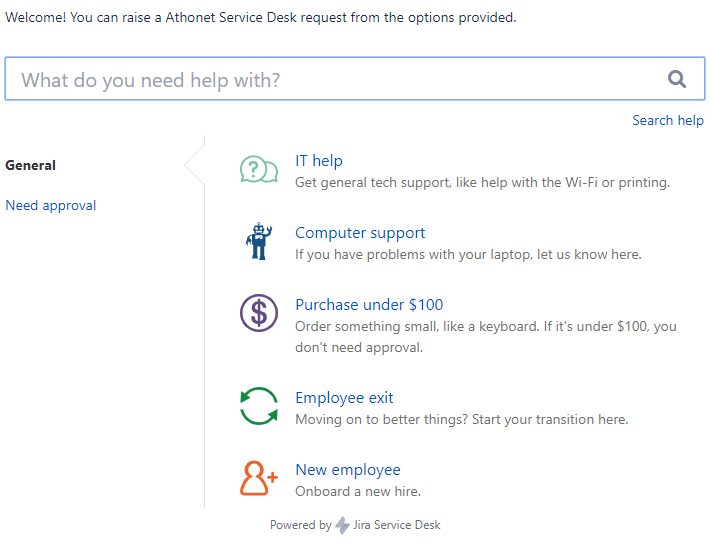
\includegraphics[width=\textwidth]{resources/Annotation2019-07-24170249}\\
		\caption{A Jira Service Desk portal}
	\end{figure}
	The installation of Confluence came after understanding all the basics of Jira and becoming familiar with it.
	For the newly installed software the H2 database was enough as for the previous one.
	Both software run on the same system, and their services are offered on port 8080 and 8090 respectively for Jira and Confluence via HTTP protocol.\\
	During the installation of Confluence, the install wizard program allowed me to insert all data of the Jira instance in order to connect them.
	A knowledge base for the Service Desk project and a documentation space for the Software project have been generated in order to test the connection.\\
	To allow a better integration between these tools, Atlassian allows to have a single database table containing the users information stored on either one of Jira or Confluence's instances.\\
	This was shown during the installation of Confluence as an option to link it with Jira's instance was presented by asking for the administrative credentials for connecting to the database and using Jira's users.
	Jira and Confluence both use the open source Apache Tomcat web server.
	This particular web server has issues regarding the login when both software run on the same IP address: each program stores \gls{cookies}\glsadd{Cookie} to allow users to log in without inserting each time username and password.
	On each log in though, users were automatically logged out of the system almost immediately.
	After a research on the Internet I found a post\cite{user-is-constantly-logged-out-of-jira} in Atlassian's blog regarding this problem: the answer was that when run on the same IP address, cookies from Jira and Confluence go in conflict.
	This post was associated with a more detailed issue\cite{JRASERVER-36960} in Jira's own portal.\\
	The solution to this problem was to change the \gls{context path}\glsadd{Context Path} of both applications\cite{how-to-change-the-jira-application-context-path} in the \Quote{server.xml} file that contains the configuration of the web server.
	An example of changing the context path is:
	\begin{center}
		\texttt{http://yourdomain.com:8080}
	\end{center}
	\vspace{-10pt}
	becomes:
	\vspace{-10pt}
	\begin{center}
		\texttt{http://yourdomain.com:8080\textbf{/jira}}
	\end{center}
	For Confluence, where the default port is 8090, the context path would become:
	\begin{center}
		\texttt{http://yourdomain.com:8090\textbf{/confluence}}
	\end{center}
	Contrary to what was said in the beginning, the tutor had communicated me that the IT department opted to maintain for using GitLab\cite{gitlab} instead of installing BitBucket\cite{bitbucket}, another Atlassian software.	
	This because GitLab was already in use by the developers, so they would not need to learn a new software that could affect their work routine.
	\begin{figure}[H]
		\centering
		\includegraphics[width=.5\textwidth]{resources/glan}\\
		\caption{GitLab Logo}
	\end{figure}
	Connecting these tools together means that a developer can interact with Jira's issues from a GitLab project by typing it's ID in the messages that he uses for commits, comments, merge requests and so on.
	GitLab's documentation has a dedicated page with instructions, examples and a guide that allow configuring both tools\cite{integrations}.\\
	This functionality allows GitLab to interact with Jira's default workflows, which sometimes are too simple for some software projects.\\
	Since the license for GitLab's hosted version is not \Quote{Premium} (or \Quote{Silver} for the online one) there is no interaction the other way around, from Jira to the repository\cite{jira_development_panel}.
	Since these tools are not strictly related, there is no direct project mapping from GitLab to Jira, a commit message in the repository may reference multiple Jira issues from different projects, so it's the programmer's discretion to comment wisely.
	Later in the text it's described the installation of a plugin that allows these tools to connect with more functionalities.\\
	A demo that touched all the previously viewed arguments was set in place for showing the progress made to the tutor.	
	Because his availability at the moment was very little, from the time the meeting was set to the actual moment of it happened, the interface of the system was customized by adding the colors of the company and its logo.
	\begin{figure}[H]
		\centering
		
\includegraphics[width=\textwidth]{resources/jira_custom}\\
		\caption{Custom menu interface for Jira}
	\end{figure}
	\vspace{-.5cm}
	\begin{figure}[H]
		\centering
		
\includegraphics[width=.85\textwidth]{resources/confluence_custom}\\
		\caption{Custom menu interface for Confluence}
	\end{figure}
	During the meeting, the tutor liked the progress that was made and asked for more elaborate mock projects for presenting the tools' combined functionalities to other company figures.\\
	The projects registered until that moment in Jira and their related spaces in Confluence were deleted and, as hinted in \ref{sec:time_planning}, a snapshot of the VM hosting the software was taken.\\
	Until this point the completely fulfilled objectives were: \textit{O01}, \textit{O02}, \textit{O05}, \textit{D03}.\\
	Although the connection between Jira and GitLab was established, to fulfill O04 it was required that GitLab supported custom workflows for Jira Software projects.
	
\section{First realistic mock projects and feedback}

	The previous paragraph marked the first three weeks of the internship.
	Starting the fourth week the task was to implement more realistic projects in Jira, connecting them to Confluence providing them with documentation and creating a link with GitLab.
	The objective was to expand the demo so that it could be shown to other members of Athonet to understand, both me and them, how these software can be used in their departments.\\
	The new Software projects created in Jira were called \Quote{EPC} and \Quote{Dashboard}, linked to their documentation spaces in Confluence, respectively \Quote{EPC Documentation} and \Quote{Dashboard Documentation}.
	To show the functionalities of Jira Service Desk as a knowledge base portal (sharing internal documents between employees), the \Quote{Athonet Internal Wiki} project was created.\\
	For the first project a more articulate workflow has been implemented to resemble the realistic evolution of an issue inside the company.
	\begin{figure}[H]
		\centering
		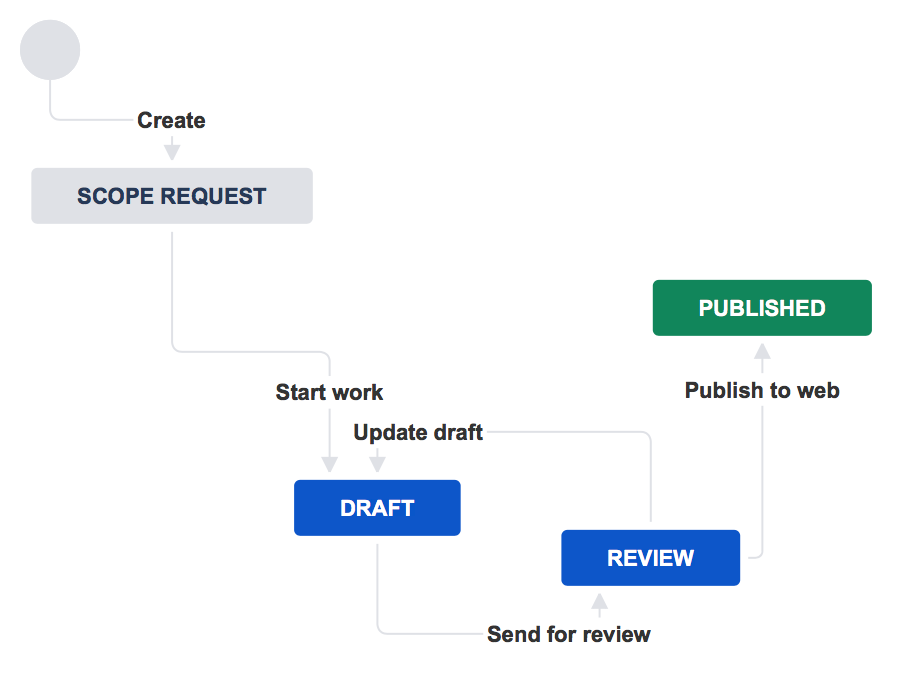
\includegraphics[width=.7\textwidth]{resources/Web+update+workflow}\\
		\caption{Custom example workflow that can be implemented in a Jira project}
	\end{figure}
	While working on the mock projects and creating issues, it was useful to note down all the most important customization that an administrative user can use to set up the software, not only for Athonet's specific purposes but in general.\\		
	To make the project more realistic three new user groups were created, besides the default ones, to which there were assigned three users each:
	\begin{itemize}
		\item Management
		\item Verification
		\item Developers
	\end{itemize}
	Every group had custom permissions allowing to demonstrate how basic security rules work in these tools (requirement \textit{D06}).\\
	A first draft of how the menu for creating a new issue can be customized was done as well, although not final (requirement \textit{D05}). 
	\begin{figure}[H]
		\centering
		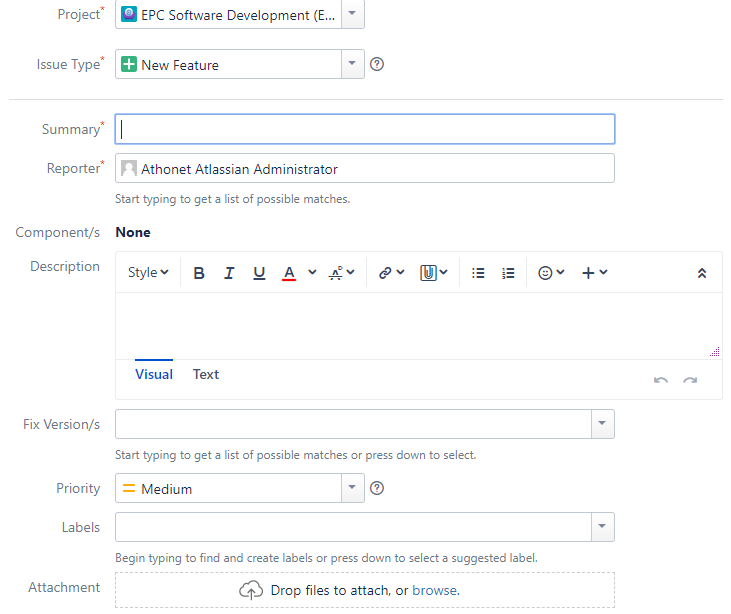
\includegraphics[width=.9\textwidth]{resources/Annotation2019-07-24170502A}\\
		\caption{Draft for custom issue creation and editing menu in Jira}
	\end{figure}
	After talking to the tutor about the made, he was able to set a meeting with himself, the verification and developer managers.
	Slides were prepared in order to explain the nomenclature in Jira, described in this document in \ref{sec:concepts}, and the features that have been paired to the demo projects.\\
	The core of this meeting was a discussion between the managers focused on understanding how their ongoing projects in Redmine could be implemented in such a way that the employees would not be forced into using a strict Agile methodology, but to accommodate and let them understand how these tools work without creating chaos.\\
	There was a discussion on how applying a strict Agile methodology could impact their time division.
	Agile provides sprints that by definition last two weeks, and these produce deliverables that bring added value to the project.
	Athonet's line of work though is focused on adding value to the product upon new releases that are scheduled differently by their purpose:
	\begin{itemize}
		\item Bug fix
		\item Minor release (for patching issues with the code or to improve performance)
		\item Major release (for new features)
	\end{itemize}
	Sprints would disrupt the routines of their developer team, the verification team and of management.
	In this case it would not be the tool that adapt to the company but vice versa the company would need to change in order to use the tool and would result counterproductive.\\
	The developer manager stated that he wanted a way to measure productivity, so I showed him the \Quote{Reports} section that is present for all kind of Jira projects.
	Here there are the burndown report charts that have been explained earlier in the text, in \ref{sec:metrics}.
	\begin{figure}[H]
		\centering
		\makebox[\textwidth][c]{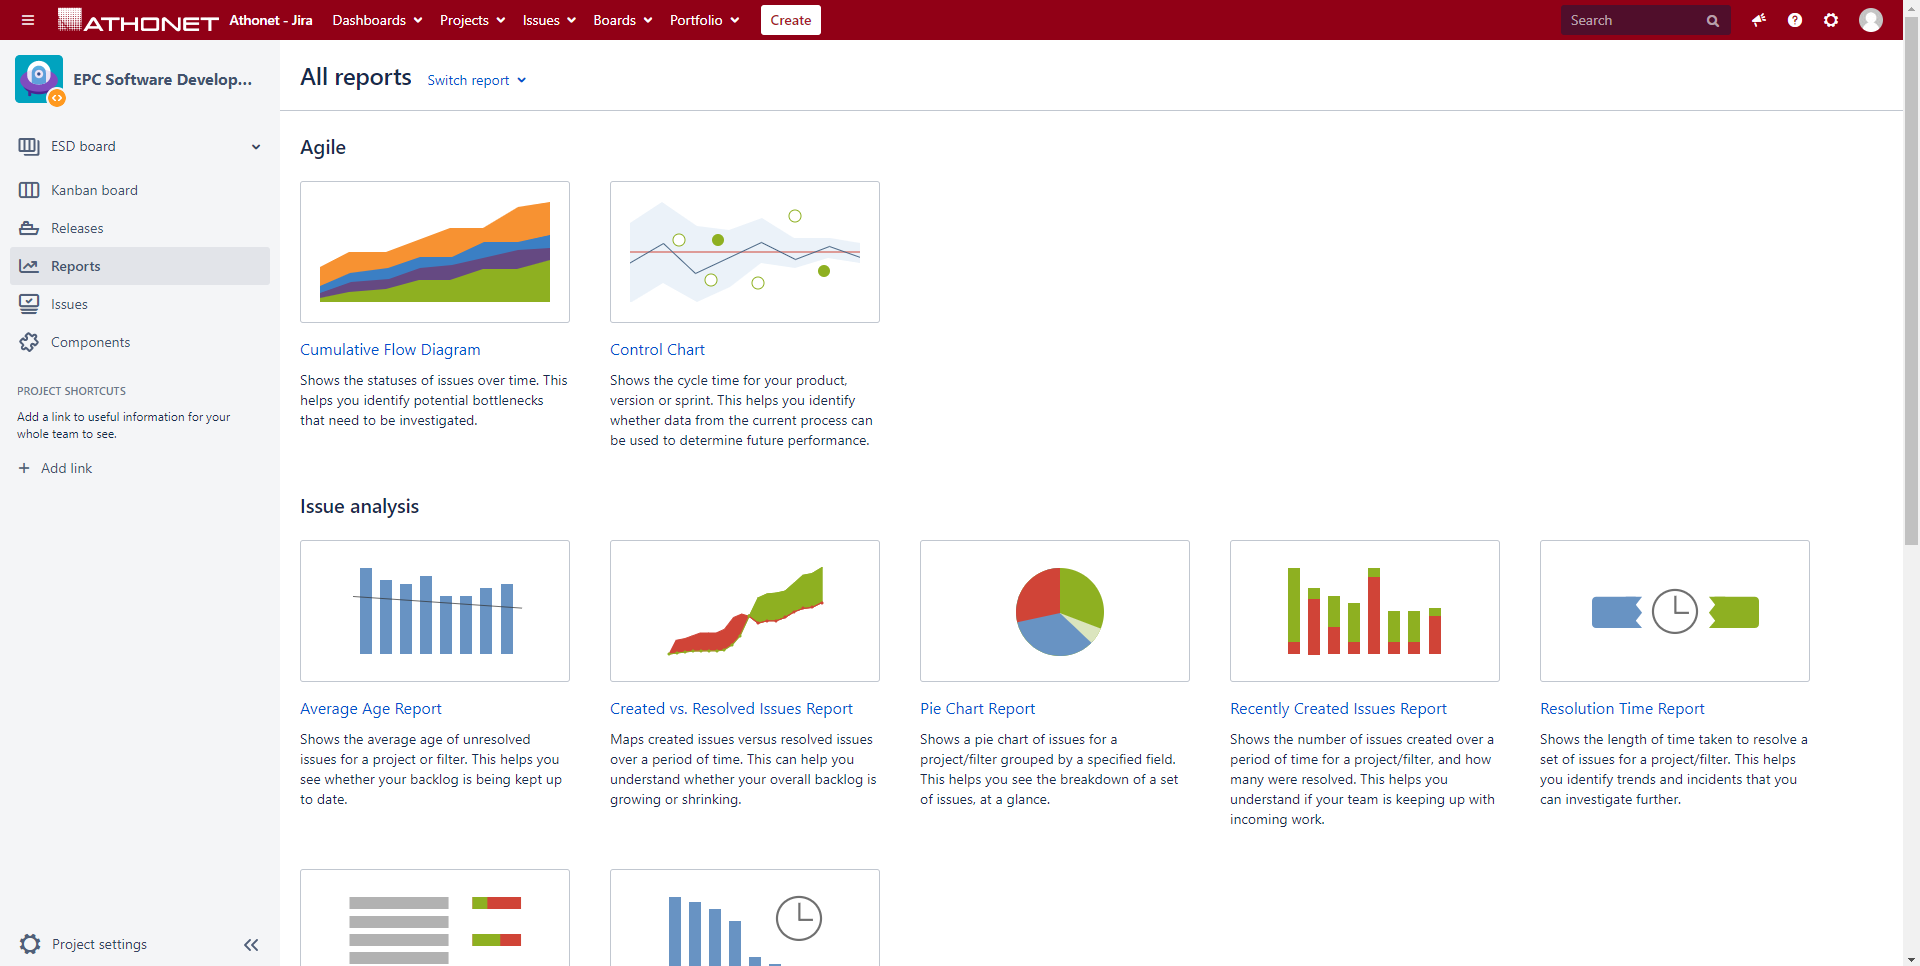
\includegraphics[width=1.2\textwidth]{resources/Annotation2019-07-24180041}}%
		\caption{Kanban board from a Jira project}
	\end{figure}
	Both managers were more pleased to see that Kanban boards resembled better their way of working, even if they want to maintain some of Scrum's peculiarities.
	The developer manager also said that it would be better for the company's way of working since developers could plan their tasks based on what has to be completed for the next release, so for a longer period of time.\\	
	This implied there would be a more particular workflow that had to be implemented and the managers were pleased to see that it could be easily done, as for customizing the issue creation and modification menu.\\
	They were also glad about the internal wiki project because it suggested there could be one single tool for both internal documentation regarding clients and general notes for employees.
	The following image is an example of how an article is visualized in this wiki.
	\begin{figure}[H]
		\centering
		\makebox[\textwidth][c]{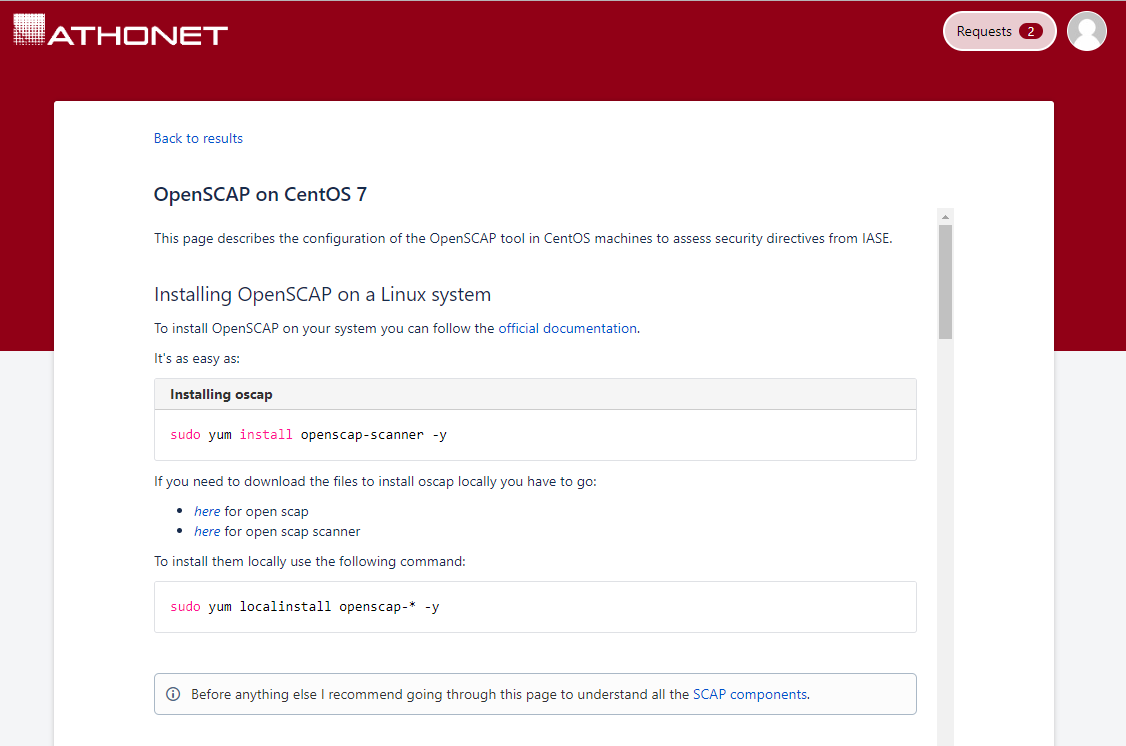
\includegraphics[width=1.1\textwidth]{resources/Annotation2019-07-2470331}}%
		\caption{Screenshot of article in Jira Service Desk}
	\end{figure}
	Articles like this correspond to pages written in a Confluence knowledge base space connected to the Service Desk project.
	\begin{figure}[H]
		\centering
		\makebox[\textwidth][c]{\includegraphics[width=1.1\textwidth]{resources/Annotation2019-07-24180113}}%
		\caption{Screenshot of a page in Confluence that is being edited}
	\end{figure}
	The company members needed time for internal discussions that had to be done in order for the managers to understand how to adapt the workflow they had in Redmine for Jira and how to include Confluence in the mix.
	In this period the documentation was elaborated, anticipating it from the original plan in the \Quote{Piano di Lavoro}.\\
	The first one to be produced was the \Quote{Installation an Configuration Guide}, written for the IT administrators and the people that would maintain, configure and eventually reinstalled if needed, the software.
	After this was drafted and approved from the tutor, I worked on the \Quote{Final User Guide}, written in the wiki Confluence that was previously demoed.
	Both regarding requirement \textit{O03}.
	Later on, a new meeting was scheduled with the product owner, who wanted to understand better Portfolio and how the concept of \Quote{product} matches the \Quote{project} denomination in Jira.\\
	Project and product sound similar and the two concepts are often confused with each other.
	A project is a temporary endeavour, with a clear definition of what needs to be delivered and by when, it has a beginning and end date.
	A product is designed to continually create value for customers by solving their problems\cite{product}.\\
	For the product owner, one of the most important things was to see how releases are mapped inside the software, since Redmine did not offer such an intuitive interface and did not allow to see them on a timeline and applying custom filters.
	He approved the progress made after seeing it and also said that he wanted the credentials to start using the software and see how to map the ongoing projects in Redmine to new ones in Jira or how to eventually migrate them, as per requirement \textit{F02}.\\
	After using it for a couple of days and talking with the other managers, he told me how they want to implement the evolution of an issue.
	Since they were not sure letting users access Service Desk directly, an employee would create an issue that would represent the customer request through service desk.
	The customer request could be a new feature, a bug report, require support, etc.
	This would then be picked up by a team that would bring it inside a Business type of project by creating a linked issue.
	This project would have a particular workflow and contains the more high lever tasks like documentation, meeting notes, feature statuses, etc.
	These shared notes and documents would be stored in Confluence, where there would be links to them.
	After they have been approved for production another team would create a linked issue inside the software project.
	This would most likely be divided in many sub-issues by the team leader and these would be visible by the developers.
	Each developer could then pick an issue to work on and handle it as he wants by, for example, dividing it in smaller sub-issues.\\
	The next week another meeting was scheduled with more company figures: a senior developer, the business strategy manage, the managers from the previous meetings, the CTO and the tutor.\\
	As in the other meetings I have presented the software, the major use cases and progress done, referencing the objectives achieved and showing them the working system by creating issues in projects that would resemble the way of working described by them.\\
	Even with the requirements changes that occurred, I was on schedule with the planning, a more detailed view can be seen in the Gantt diagram in \ref{gantt_2}.
	\newpage
	\begin{landscape}
		\vspace*{\fill}
		\begin{figure}[H]
			\centering
			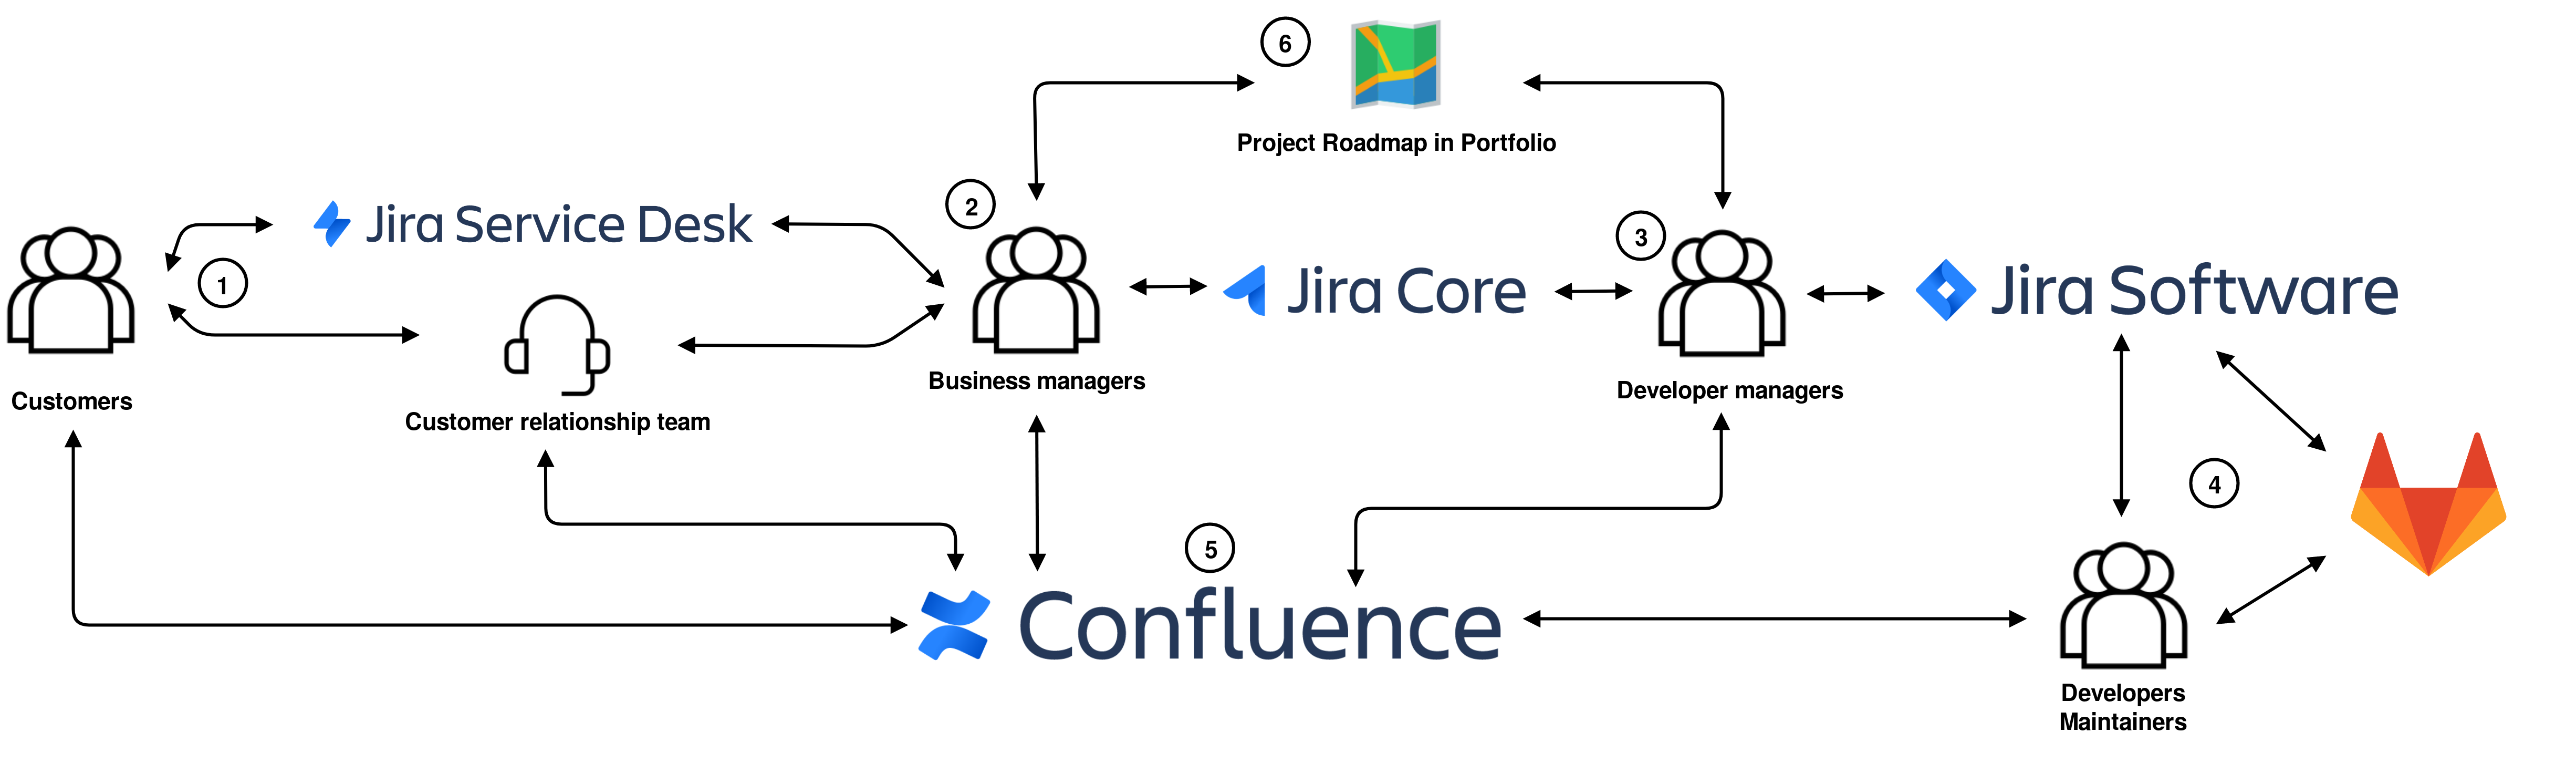
\includegraphics[width=22cm]{resources/UntitledDiagrammmmm}\\
			\caption{Evolution and transitioning of an issue}
		\end{figure}
		The main steps that an issue passes are:
		\begin{enumerate}
			\item The customer reports a bug or feature request to the Customer Relationship team or through a Jira Service Desk project
			\item The request is then picked up by the Business managers that discuss it and link it to a Jira Core issue in a dedicated project
			\item The features that are ready to be developed are sent in the Jira Software project by the development team managers
			\item The developers choose what to work on and commit to GitLab, which is connected with Jira Software, using special keywords
			\item Confluence is fully connected with every other Atlassian tool and allows users to store notes and documents
			\item Jira's Portfolio plugin is always up to date with the status of the issues and can be consulted by the managers (or developers)
		\end{enumerate}
		\hfill
		\vspace*{\fill}
	\end{landscape}
	\newpage

\section{Transitioning into Production and final feedback}

	To better connect GitLab with Jira the plugin \Quote{GitLab Listener}\cite{gitlab-listener} was installed.
	This allows for wider connectivity between the two products supporting custom workflows and more transitions with commit messages like:
	\begin{center}
		\texttt{New version \#refs ALLGEN-12 GTTSLT-2 \#time 1h 15m \#action ToDone}
	\end{center}
	This kind of command references two issues in two different Jira projects, telling the time spent and transitioning both to the \Quote{Done} column.
	Installing this plugin allowed to completely fulfill requirement \textit{O04}.
	\begin{figure}[H]
		\centering
		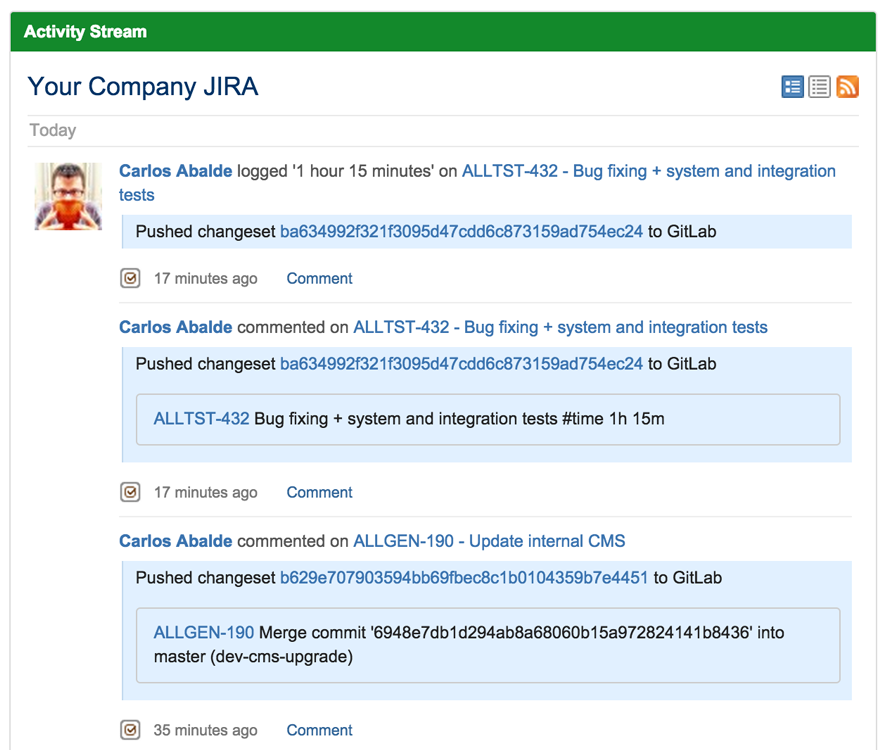
\includegraphics[width=.7\textwidth]{resources/aiaiai}\\
		\caption[Screenshot of how GitLab's messages are seen in Jira's interface]{Screenshot of how GitLab's messages are seen in Jira's interface\cite{gitlab-listener}}
	\end{figure}
	Although in the first planning this was a longer period of time, this last phase was shortened.
	This was due because of the many internal discussions that took place for the software to be approved and for the various managers of the departments to understand how to introduce it to their subordinates.\\
	After the last meeting, described in the previous paragraph, new users were created for the managers that participated and the credentials were given so that they could see the interface and interact with the mock projects that remained there.\\
	The tutor had credentials as well and he was very enthusiast of how the demo performed and the potentials of the software, although this had to be well understood by the other managers and members of the company as well.\\
	Although the last snapshot of the VM that was made contained a working infrastructure ready to be moved in a production environment, the IT department opted to wait until they understood how to properly secure the server that was going to host it.
	The most important part would be creating a secure \gls{VPN tunnel}\glsadd{VPN} that would allow employees that are working from other locations outside the company to connect as if they would be inside the building.
	This method must ensure thought that there would be no possibility for any other to get, or even hack, inside the company's network and access their products' source code.
	Besides this, the other managers where glad to hear that the tools have been approved and where happy about the demonstration.\\
	Because of this restrictions from the IT department, some of the requirements could not be fulfilled: \textit{D01}, \textit{D04}, \textit{F01}, \textit{F02}.
	These requirements could not be fulfilled because of the restrictions imposed by the IT department for interns.\\
	It would have required me to access their production server and having access to the data that is contained in the Redmine instance, which is available only for the employees.
	Or in case of \textit{D01} I could not fulfill the requirement because I would have needed access to the administrative passwords of Office 365.\\
	Requirement \textit{D02} was not fulfilled because while going on with the project, the tutor noted that there was no need for custom scripts.
	
\section{How are these tools being used}
	Even if Athonet does go for a pure Agile development model, the tools it has chosen to use still help to improve the organization of their work.
	In fact, the tools fits their current needs, which reflect an hybrid model between Scrum and Kanban: \Quote{Scrumban}.
	As in Kanban it helps visualizing workflow, limiting work in process (WIP), and measuring productivity are prioritized.	
	Scrumban removes the practice of limiting WIP by time (i.e. velocity and Sprint boundary) and replaces it by limiting WIP for each stage.
	It's based on having a continuous flow of work, which is what Athonet has for their products.\\
	In Jira, this methodology is called \Quote{Kanplan}\cite{kanplan}, and it is well documented on the \Quote{Agile Coach} section on their website.
	%!TEX root = ../thesis.tex
\chapter{Conclusions}
\label{conclusions}

After having explained how this solution has been implemented, I would like to draw the conclusions on the project, internship experience and knowledge acquired.

\section{Objectives achievement}
	Even thought the original objectives have changes during the internship, the software's documentation and the blogs presented contained the correct answers in order to correctly configure the software.\\
	Here is a list of the requirements and their status at the end of the project:
	\begin{itemize}
		\item \underline{\textit{O01}}: ACHIEVED
		\item \underline{\textit{O02}}: ACHIEVED
		\item \underline{\textit{O03}}: ACHIEVED
		\item \underline{\textit{O04}}: ACHIEVED
		\item \underline{\textit{O05}}: ACHIEVED
		\item \underline{\textit{D01}}: NOT IMPLEMENTED
		\item \underline{\textit{D02}}: NOT IMPLEMENTED
		\item \underline{\textit{D03}}: ACHIEVED
		\item \underline{\textit{D04}}: NOT IMPLEMENTED
		\item \underline{\textit{D05}}: ACHIEVED
		\item \underline{\textit{D06}}: ACHIEVED
		\item \underline{\textit{F01}}: NOT IMPLEMENTED
		\item \underline{\textit{F02}}: NOT IMPLEMENTED
	\end{itemize} 
	Note that the ones with \Quote{NOT IMPLEMENTED} status is because of internal rules that would not allow interns to interact with the production environment.\\
	Although these have not been achieved, the knowledge on how to implement them has been acquired since their description is contained in the documentation that has been left in Athonet.

\section{Improvement and future implementations}
	As many other projects there are many improvements that can applied.
	To complete the project presented in this thesis I would move it into a production environment and migrate the data from the Redmine instance.
	To have a better and more stable environment thought, there are various improvements that could be made.
	The first and most important one, in my personal opinion, would be separating the database from the Virtual Machine that hosts the software.
	This would bring advantages like: 
	\begin{itemize}
		\item the machine with Jira and Confluence would be less stressed since it would not have so many reads and writes per disk
		\item the database could be stores in a single machine (or multiple ones) with dedicated disks arranged in a redundant way which adds a layer of security, in a disaster recovery plan, over regular backups
		\item maintenance to either one of the machines would be easier and would impact less the company's work
		\item etc.
	\end{itemize}
	Another important improvement would be separating the Confluence instance from the Jira one and, instead of having them running on a dedicated Virtual Machine each, creating a Docker \cite{dock} \gls{container}\glsadd{Container} so that they would be easier to handle (copy, migrate, update).
	\begin{figure}[H]
		\centering
		\includegraphics[width=.4\textwidth]{resources/docker}\\
		\caption{Docker logo}
	\end{figure}
	The use of containers would also allow a better usage of the host machine's resources like memory and CPU power by sharing them.
	These would otherwise be split and left unused by the VMs.
	This kind of improvements should be implemented when planning the migration of the services in a production environment.\\
	Other future improvements can be installing plugins that would allow connectivity with the Microsoft Office suite allowing employees to produce documents and reports without learning how to do it in Confluence and just uploading them.

\section{What I have learned}
	During this internship I had the possibility to better understand the hierarchy of a company, an argument well introduced in the Software Engineering (SWE) course.
	In Athonet I had the possibility to see this first hand and to interact with people on more levels of responsibility, from the CTO, to the product owner to the managers of verification and development teams.\\
	About the tools, it is important to know how to use software like this not only for tracking the status of issues but on how to see other information about them as well.
	This kind of tools are are found in many IT companies, small or big, since they ease not only the work of keeping track of issues but the documentation of meeting notes, internal documents, release changelogs and many other features as well.\\
	In a growing company like Athonet it is useful to set some boundaries, not only for lower level employees like developers, but for the management as well.
	%!TEX root = ../thesis.tex
\renewcommand\thechapter{A}
\chapter{Appendix A: Gantt Diagrams}
\label{AppendixA}

This Appendix contains the ...

%todo rivedere titoli
\begin{landscape}
	\vspace*{\fill}
	\section{GANTT 1}
	\label{gantt_1}
	\begin{figure}[H]
		\centering
		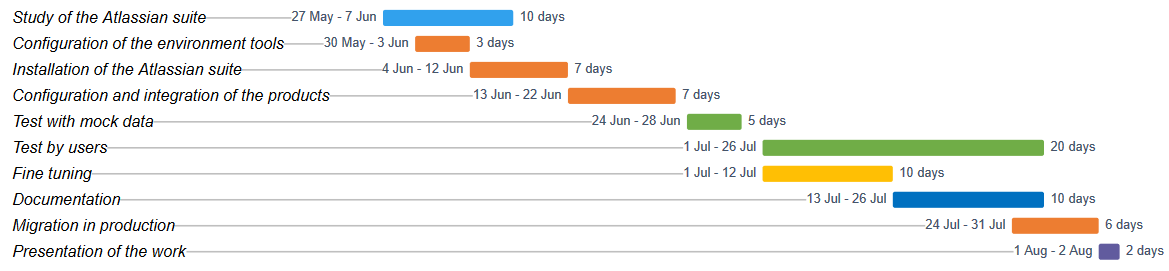
\includegraphics[width=22cm]{resources/work_plan_gantt}\\
		\caption{Gantt diagram contained in the ``\textit{Piano di Lavoro}'' document}
	\end{figure}
	\vspace*{\fill}
\end{landscape}
\newpage
\begin{landscape}
	\vspace*{\fill}
	\section{GANTT 1}
	\label{gantt_2}
	\begin{figure}[H]
		\centering
		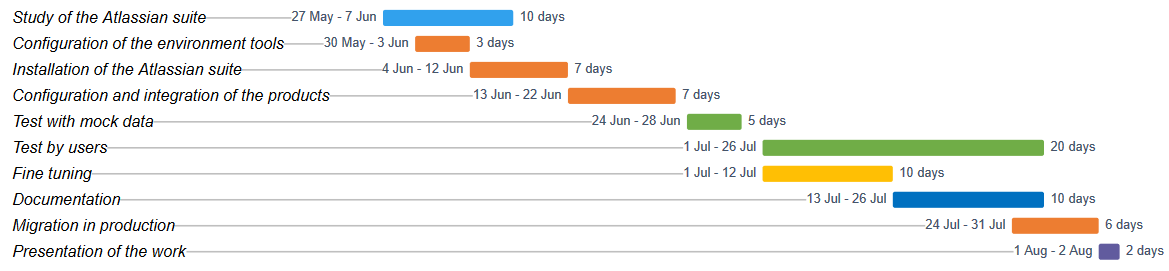
\includegraphics[width=22cm]{resources/work_plan_gantt}\\
		\caption{Gantt diagram contained in the ``\textit{Piano di Lavoro}'' document}
	\end{figure}
	\vspace*{\fill}
\end{landscape}
	%!TEX root = ../thesis.tex
\renewcommand\thechapter{B}
\chapter{Appendix B: Project requirements}
\label{AppendixB}

\hl{ADD COMPLETE TABLE WITH THE PROJECT REQUIREMENTS}

\begin{center}
	\begin{tabular}{ |c|c|c| } 
		\hline
		cell1 & cell2 & cell3 \\ 
		cell4 & cell5 & cell6 \\ 
		cell7 & cell8 & cell9 \\ 
		\hline
	\end{tabular}
\end{center}


	
	\addcontentsline{toc}{chapter}{References}
	\bibliography{references}
%	\cleardoublepage
%	\phantomsection
%	\addcontentsline{toc}{chapter}{Acknowledgments}
%	\acknowledgments
	
	\cleardoublepage
	\phantomsection
	\addcontentsline{toc}{chapter}{Glossary}	
	\glsaddall
	\printglossary

\end{document}